% !TEX program = pdflatex --shell-escape

\documentclass[11pt]{article}
\usepackage[round,sort&compress,semicolon]{natbib}
\usepackage{times}
\usepackage[T1]{fontenc}
\usepackage[utf8]{inputenc}
\usepackage[pdftex]{graphicx}\usepackage[letterpaper, left=1.0in, right=1.0in, top=1.0in, bottom=1.0in]{geometry}
\usepackage{ragged2e}
\usepackage{url}
\usepackage{setspace}
\usepackage{lineno}
\usepackage{multirow}
\usepackage{pdflscape}
\usepackage[backref=page]{hyperref}
\usepackage{rotating}
\usepackage{booktabs}
\usepackage[hypcap, labelsep=period, labelfont=bf]{caption}
\usepackage{array}
\usepackage{color}
\usepackage{soul}
\usepackage{mathtools}
\usepackage{pdflscape}

\usepackage{amsmath}
\usepackage{amsfonts}       % blackboard math symbols
\usepackage{nicefrac}       % compact symbols for 1/2, etc.
\usepackage{microtype}      % microtypography
\usepackage{doi}


\usepackage[dvipsnames,svgnames,table]{xcolor}
\urlstyle{same}
\setlength{\RaggedRightParindent}{\parindent}
\linenumbers
\linespread{1.5}

% restart counting in the supplement
\newcommand{\beginsupplement}{%
	\setcounter{table}{0}
	\setcounter{figure}{0}
	% \setcounter{section}{0}
	% \setcounter{subsection}{0}	
	\renewcommand{\thetable}{S\arabic{table}}%
	\renewcommand{\thefigure}{S\arabic{figure}}%
	% \renewcommand{\thesection}{S\arabic{section}}%
	% \renewcommand{\thesubsection}{S\arabic{section}.\arabic{subsection}}%          
}

%%% Add PDF metadata to help others organize their library
%%% Once the PDF is generated, you can check the metadata with
%%% $ pdfinfo template.pdf
\hypersetup{
     colorlinks   = true,
     citecolor    = Indigo,
     linkcolor    = DarkCyan,
}

\begin{document}

\begin{center}
	{\bf \Large
	% Redrawing the Boundaries of North American \emph{Delphinium}: Geography and Admixture 
	% Geography and Admixture Shape the Genome-Scale Phylogeny \\[0.2cm]
	% of North American \emph{Delphinium}
	% Towards a comprehensive phylogeny of North American \\
	% \emph{Delphinium} (Ranunculaceae)
	% Phylogenomic Evidence for Taxonomic Reevaluation in North American
	% \textit{Delphinium} and the Dominance of Geographic Patterns}\\[0.5cm]
	% Phylogenomic Evidence for a Major Taxonomic Revision of North American
	% \textit{Delphinium} and the Dominance of Geographic Patterns}\\[0.5cm]
	Geography and Admixture Shape the Genome-scale Phylogeny of \\
	North American \emph{Delphinium}\\[0.5cm]
	}

Jared B. Meek$^{1,*}$, Daniel Cook$^2$, B. Shaun Bushman$^3$, Kim Thorsted$^3$, Deren A.R. Eaton$^{1,*}$\\[0.5cm]

1. Department of Ecology, Evolution, and Environmental Biology, Columbia University, 1200 Amsterdam Ave, New York, NY, 10027, USA;\\
2. USDA-ARS Poisonous Plant Research Laboratory, 1150 E 1400 N Logan, UT, 84341, USA;\\ 3. Forage \& Range Research Lab, Utah State University, Logan, UT 84322, USA;\\ 
* Corresponding Authors: jared.meek@columbia.edu; de2356@columbia.edu
% daniel.cook@usda.gov\\
% shaun.bushman@usda.gov\\

% https://orcid.org/0000-0002-5922-2770  D.E.
% https://orcid.org/0000-0001-8191-4266  J.M.
% https://orcid.org/0000-0001-8568-113X  D.C.


\end{center}

Keywords: Larkspur, Hybridization, Plant, Syngameon, Alpine, RAD-seq, Biogeography

\RaggedRight

\section*{Summary}

The genus \emph{Delphinium} exemplifies the complexity of plant diversification in mountainous regions, where rapid speciation, hybridization, and morphological convergence frequently obscure species boundaries. The North American lineage \emph{Delphinium} sect. \emph{Diedropetala} has rapidly radiated across a range of ecological habitats, from alpine tundra to desert grasslands, forming an iconic component of western wild flower communities. Despite decades of taxonomic study, phylogenetic relationships within this group remain poorly resolved. Here, we present a genome-scale phylogeny of 34 taxa using ddRAD-seq data from 150 individuals sampled across their geographic ranges. Our results reveal strong phylogenetic structure corresponding to biogeographic regions, including several well-supported clades that cut across existing taxonomic subsections, emphasizing the need for taxonomic revision. Hybridization and introgression are widespread, occurring both within and between these regional clades. Most species are connected through a syngameon-like network of introgression, with few widespread species acting as central hubs. We describe six higher-level clade names and use an agent-based artificial intelligence analysis to identify morphological synapomorphies that align with our genomic findings. Our study demonstrates that geography and gene flow have played a dominant role in shaping the evolutionary history of \emph{Delphinium}, offering a framework for revising its taxonomy and informing future conservation efforts.


\section*{Introduction}
% Western North America contains unresolved plant clades that we need to understand better
Western North America harbors exceptional topographic and ecological heterogeneity
that has shaped the diversification of many endemic plant lineages.
% fostered
% North America is a topographically and ecologically complex region that has fostered the
% diversification of many endemic plant lineages. 
Its flora includes numerous rare and specialized taxa narrowly distributed
along climatic gradients, many of which now face mounting threats from shifting
climate and precipitation patterns, increased wildfire frequency, and habitat loss
\citep{kannenberg_rapid_2021,overpeck_climate_2020}.
% 
% Although it is among the most thoroughly studied botanical areas in the world
Although North America is among the best-studied floras globally
 \citep{hickman1993jepson,FNA_Vol3_1997,cronquist_intermountain_1984}, 
persistent taxonomic uncertainties continue to
impede efforts to quantify biodiversity and track its decline. 
% out ability to accurately quantify biodiversity and track its decline. 
% 
% Improved taxonomic knowledge is essential to detect 
These knowledge gaps limit our ability to detect 
local extinctions \citep{wiens_climate-related_2016},
estimate species range shifts \citep{frei_plant_2010}, 
and prioritize conservation actions.
% and scale ecological predictions across spatial hierarchies. 


The delimitation of species and their phylogenetic relationships remains poorly
understood even within some of the most enigmatic plant lineages of this region, 
including 
larkspurs \citep[\emph{Delphinium};][]{jabbour_phylogeny_2012, xiang_recircumscription_2017}, 
beardtongues \citep[\emph{Penstemon};][]{wessinger_multiplexed_2016,wolfe_phylogenetics_2021},
and paintbrushes \citep[\emph{Castilleja;}][]{tank_phylogenetic_2009,jacobs_quantifying_2019}.
% 
% Species-rich lineages are often taxonomically challenging due to their
% rapid diversification and high frequency for hybridization.
%Species-rich lineages often present taxonomic challenges caused by their 
%rapid diversification and high frequency of hybridization.
% 
This is especially true within applications of morphological systematics, where lineages
may be under- or over-split in relation to their rates of morphological evolution.
% 
In montane regions, these rates can vary considerably. Geographically isolated
populations or species are prone to under-counting when they exhibit parallel
evolution or cryptic variation
\citep[e.g.,][]{donoghue_replicated_2022}; 
whereas taxa may be over-split when populations exhibit extensive environmental
plasticity, or stable hybrid phenotypes \citep{divittorio_natural_2020}.
% 
% This problem can be exacerbated in montane lineages, where cryptic variation may
% exist between geographically isolated populations,  may be 
% be overlooked 
% This problem is likely exacerbated in montane lineages, where geographically isolated populations or species exposed to similar environmental gradients can exhibit similar 
% morphologies arising from plasticity or parallel adaptations
% 
% Such patterns may be exacerbated in mountainous regions, where parallel adaptations
% to similar environmental gradients cause cryptic variation, as in the case of 
% \emph{Viburnum} in neotropical cloud forests \citep{donoghue_replicated_2022}. 
% 
% When selection maintains distinct morphologies across environmental gradients, 
% as in the case of desert \emph{Encelia} \citep{divittorio_natural_2020}, rare but 
% distinct phenotypes that arise in hybrid populations can lead to inflated species 
% descriptions.
% 
Integrative systematic studies that incorporate phylogenomic evidence alongside
morphological and geographic information can better assess the distinctiveness of
taxa, especially in lineages characterized by hybridization, plasticity, and 
parallelism \citep[e.g.,][]{donoghue_replicated_2022,hipp_genomic_2020}.
% 
Such work contributes not only to improving plant taxonomy and biodiversity
research, but also to detecting associations between environments and the evolution or expression of unique phenotypes \citep{anstett_regional_2021, gross_unforeseen_2024,melton_draft_2021}.

% Such integrative studies contribute not only to improving plant taxonomy
% and biodiversity research, but also identifying and understanding the 
% ...
% This work contributes not only to improving plant taxonomy, but also to
% our ability to quantify and preserve biodiversity; identify historical 
% corridors of migration and dispersal; and investigate plant adaptations
% to extreme conditions hipp_genomic_2020


A prime example of these dynamics is the North American clade  \emph{Delphinium} 
sect. \emph{Diedropetala} \textcolor{red}{Huth. After originating in the Himalaya-Hengduan region of Asia \textasciitilde~32 Ma, \emph{Delphinium} L. diversified into 650-700 species, speciating both west (through Eurasia, the Mediterranean, and into Africa) and east, arriving in western North America \textasciitilde~3 Ma, where it rapidly radiated into approximately 60 species} \citep{jabbour_phylogeny_2012}.
% 
\textcolor{red}{While \emph{Delphinium} exhibits both annual and perennial life cycles, all} species of th\textcolor{red}{e North American sect. \emph{Diedropetala}} are perennial herbaceous plants characterized by large 
showy flowers that are typically blue and purple, and less commonly red, yellow, 
or white. 
% 
Many species are widespread and abundant in montane, grassland, and desert habitats,
while others exist as narrow endemics that have specialized adaptations to harsh 
alpine environments \citep{warnock_taxonomic_1995}. 
% 
Multiple species are currently endangered in North America. 
They are economically important as ornamentals, and intensely studied for 
their toxicity to livestock \citep{cook_biogeographical_2009, 
cook_two_2017, gardner_taxonomic_2002, pfister_grazing_2014}.
% Cook et al., 2009, 2017; Gardner et al., 2002; Pfister et al., 2014). 
Their rapid diversification in North America has been attributed to dispersal and 
isolation in the various mountain ranges of the western Cordillera, especially the
Cascades, Sierra Nevada, and Rocky Mountains \citep{warnock_taxonomic_1995}.
% 
Despite multiple taxonomic and phylogenetic research efforts focused on this clade,
there is no fully resolved phylogeny of \emph{Delphinium} sect. \emph{Diedropetala},
and little is known about its biogeographic history across western North America.


The genus \emph{Delphinium} is often considered taxonomically difficult due to a 
limited number of 
%distinguishable 
distinguishing
morphological characters. Two comprehensive 
taxonomic treatments for North American \emph{Delphinium} have been published over 
the last century which recognize between 60-80 species, but disagree over their
exact number, nomenclature, and distribution. 
% 
In the first published circumscription of the clade, \cite{ewan_synopsis_1945}
combined extensive 
fieldwork and study of herbarium specimens to distinguish 79 species grouped 
into 13 “series” based on seed morphology, leaf architecture and pubescence, 
corolla color, and other anatomical features. 
% 
Fifty years later, Warnock’s treatment \citep{warnock_taxonomic_1995}
reduced the number of species 
from 79 to 61, comprising two sections: \emph{Elatopsis} Huth, represented by a garden 
cultivar (\emph{Delphinium elatum} L.) introduced from Europe, and 
\emph{Diedropetala}, which is composed of nine subsections.
%
These subsections are largely delineated by root structure and size, 
sepal color and length, seed morphology, and fruit position.
% 
This treatment is included in the current Flora of North America
\citep[FNA;][]{Warnock_1997_FNA_Delphinium}, and we will refer to it hereafter as 
the FNA treatment.
Other notable regional treatments of \emph{Delphinium} sect. \emph{Diedropetala} include:
\cite{rydberg_delphinium_1899, ewan_genus_1942, wilde1931studies, cronquist_intermountain_1984, ackerfield_flora_2022, chambers_comments_2018, lewis_taxonomic_1954,koontz_delphinium_2012,WeberWittmann2012,holmgren2012intermountain}.

% In addition, t
Two molecular phylogenetic studies have used
Sanger sequencing markers to examine relationships within 
section \emph{Diedropetala}.
A study by \citet{koontz_using_2004} sampled sixty-two species of 
North American \emph{Delphinium} but found that few relationships can
be resolved using a small number of molecular markers. 
% 
A deeper-scale phylogenetic analysis by \cite{jabbour_phylogeny_2012} 
sampled a third of the North American species, as well as many other
species from across its global distribution.
Their results support section \emph{Diedropetala} as a monophyletic 
clade, but similarly lacked support to confidently 
resolve many relationships within it. \textcolor{red}{While more recent molecular studies exist for \textit{Delphinium} clades in east Africa \citep{Chartier2016}, the Mediterranean \citep{xiang_recircumscription_2017}, Russia \citep{Kashinetal2021}, and China \citep{Song2024},} no study has yet brought genome-scale data to bear on phylogenetic 
relationships within \emph{Delphinium} sect. \textit{Diedropetala} \textcolor{red}{in North America}.

% A paragraph about hybridization and the power of genomic data to resolve
Multi-locus phylogenomic analyses offer an advantage not only for inferring
species tree relationships from among discordant (conflicting) phylogenetic signals, 
but additionally for the potential to test for evidence of hybrid introgression
\citep{kubatko_species_2023, durand_testing_2011, eaton_historical_2015}.
% 
Hybridization is likely to have played a significant role throughout the 
diversification of \emph{Delphinium}. 
Many putative hybrids have been described based on morphological descriptions 
\citep{ewan_synopsis_1945, warnock_taxonomic_1995, legro_species_1961, koontz_hybrid_2001},
but the extent to which they contribute to introgressive gene 
flow between species remains unknown. \textcolor{red}{Our primary objectives in this study were to use genome-wide data to resolve the backbone of \emph{Delphinium} sect. 
\emph{Diedropetala} and investigate the extent to which widespread hybridization and introgession has contributed to its diversification throughout North America. To achieve this,} we generated a new reduced-representation genomic dataset to 
investigate phylogeny and introgression across \emph{Delphinium} sect. 
\emph{Diedropetala}.
% 
We present a new and highly revised phylogenomic hypothesis for relationships
among species representing all previously described subsections in this 
group, and discuss our confidence in this result with regard to our 
extensive sampling of populations within species, tests for hybrid 
introgression, and the biogeographic concordance of our results.



%%%%%%%%%%%%%%%%%%%%%%%%%%%%%%%%%%%%%%%%%%%%%%%%%%%%%%%%%%%%%%%%%%%%%%%%%%%%%%%%%%%%%%%%%%%
%%%%%%%%%%%%%%%%%%%%%%%%%%%%%%%%%%%%%%%%%%%%%%%%%%%%%%%%%%%%%%%%%%%%%%%%%%%%%%%%%%%%%%%%%%%
%%%%%%%%%%%%%%%%%%%%%%%%%%%%%%%%%%%%%%%%%%%%%%%%%%%%%%%%%%%%%%%%%%%%%%%%%%%%%%%%%%%%%%%%%%%
%%%%%%%%%%%%%%%%%%%%%%%%%%%%%%%%%%%%%%%%%%%%%%%%%%%%%%%%%%%%%%%%%%%%%%%%%%%%%%%%%%%%%%%%%%%
\section{Materials and Methods}

\subsection{Taxon sampling}
We collected voucher specimens and silica-preserved leaf samples during field expeditions
between 2019-2024. Additional samples were provided by the USDA Poisonous Plant Research
Lab as part of a long-term research program concerning toxicity in \emph{Delphinium}, where
tissues were stored freeze-dried.
% 
This dataset includes 150 individuals, with replicate samples of 34 \emph{Delphinium} 
taxa collected from multiple geographically disjunct populations. \textcolor{red}{When possible, we collected species from their type localities, and our sampling includes
at least one taxon as a representative of each subsection in the FNA treatment of
\emph{Delphinium}, including the type specimen for subsections \emph{Bicoloria} (Rydberg) N. I. Malyutin, \emph{Exaltata} 
N. I. Malyutin, \emph{Multiplex} M. J. Warnock, and \emph{Subscaposa} Ewan.}
We included samples from two \emph{Aconitum} L. species as outgroups.
All collections have associated geographic coordinates (Table S1) and voucher 
specimens available at the USDA Poisonous Plant Research Lab Herbarium (PPRL)
in Logan, UT.

\subsection{DNA sequencing and bioinformatics}
Genomic DNA was extracted from lyophilized leaf tissue using the Quick DNA
extraction kit (Zymo Research) adapted to a 96-well format. 
DNA quantity and quality were assessed using a spectrophotometer, TapeStation 
(Agilent), and gel electrophoresis, and genomic DNA was standardized to 20 ng/ul. 
% 
Genomic double-digest restriction-site associated DNA \citep[ddRAD-seq;][]{peterson_double_2012}
libraries were prepared at the USDA Forage \& Range Research Lab at 
Utah State University using the PstI and MspI restriction enzymes
\citep{poland_development_2012},
followed by adapter ligation, sample pooling, and a final purification
and partial polymerase chain reaction conducted for 16 cycles. 
% 
The pooled library was sequenced on an Illumina Nextseq 2000 at the Utah State 
University Center for Integrated Biosystems (Logan, UT) to produce single-end
75bp reads. 
% 
Sequence data for all samples was assembled in \emph{ipyrad} 
v.0.9.104 \citep{eaton_ipyrad_2020} using the \emph{de novo} 
pipeline and default parameter settings, except for the following
changes: datatype=ddrad, restriction\_overhang=(`TGCAG',`'),
filter\_adapters=2, maxdepth=10000, max\_SNPs\_locus=0.4,
max\_shared\_Hs\_locus=6, and max\_alleles\_consens=4. 
% 
Additional downstream analyses 
%were performed in reproducible jupyter notebooks using 
used the \emph{ipyrad-analysis} toolkit to subsample and convert data to the
appropriate format for various analysis tools while also examining the impact of
missing data.
% We then ran steps 2-7 of ipyrad to create output files for downstream analyses,
% which were performed in reproducible jupyter notebooks using the 
% \emph{ipyrad-analysis} toolkit.

\subsection{Phylogenetic inference}
\textcolor{red}{
We inferred phylogenetic relationships at both the individual and population-level using multiple inference methods, including concatenation, SNP-based, and gene-tree based.} 
%
We generated two concatenated supermatrix datasets comprising either
all loci shared across at least four samples (`min4' dataset) or 
ten samples (`min10' dataset), using the \emph{ipyrad-analysis} 
‘window\_extracter’ tool \citep{eaton_ipyrad_2020}.
%
For each dataset we inferred a maximum likelihood phylogenetic tree in
\emph{raxml-ng} v.1.2.2 \citep{kozlov_raxml-ng_2019} using the GTR+G substitution
model with four rate categories, starting from 10 random and 10 parsimony 
starting trees, and with 200 non-parametric bootstrap replicates. 
%
Because concatenation can lead to biased inference in the presence of incomplete
lineage sorting, 
\textcolor{red}{
we also employed species tree inference approaches.
First,} we inferred a species tree from each dataset using 
\emph{caster} v.1.19 \citep{doi:10.1126/science.adk9688}, a SNP-based approach 
for inferring species trees from quartet relationships.
We used the `caster-site’ method which scores topologies for each site pattern 
shared among four taxa and infers a phylogeny by combining the quartet
trees with highest support. We set the chunk size parameter to 500 
and designated for it to incorporate heterozygous variant calls.
Support was assessed from 1000 local block bootstraps. 

To achieve a "population-level" phylogeny we additionally ran caster using the same
settings as above but with a mapping file to assign individuals to populations.
We included 41 populations, where each represents a unique clade corresponding to a taxon name
that was consistently recovered as monophyletic in all phylogenetic analyses. 
Two clades did not meet this criterion.
We assigned the outgroup sample Acol2-3 to \emph{A. delphiniifolium} D.C. even though
it consistently groups with low support between the two outgroup clades. 
We assigned the sample Dalp4-2 to \emph{D. ramosum} Rydberg population 4-10, 
since it consistently groups within that clade, despite being initially 
determined as \emph{D. alpestre} Rydberg.

\textcolor{red}{
We also inferred individual gene trees for RAD-seq loci to use as input to the species tree program
Astral IV v1.23.4.6 \citep{zhang}. 
For this analysis, we selected a subset of individuals that had the greatest 
number of assembled loci from each of the 41 populations identified above. 
This allowed us to select a subset of loci that were shared across these samples and 
contained sufficient information for gene tree inference.
For these samples we used the \emph{ipyrad-analysis} ‘tree\_slider’ tool to select all loci that
contained at least 10 samples from this subset, and a minimum of five variant sites 
after pruning all other samples. For each locus, we inferred an ML tree in raxml-ng as described 
above. We collapsed all edges with bootstrap support <50\%, and input the set of trees to ASTRAL 
to infer a species tree under default settings.
}
The Python package \emph{toytree} \citep{eaton_toytree_2020} was used to collapse low support edges, 
compute tree distance metrics, and visualize trees.

% To investigate the impact of missing data on phylogenetic inference 
% we generated supermatrices from all loci shared across at least four 
% samples (`min4' dataset) or ten samples (`min10' dataset), using the
% \emph{ipyrad-analysis} ‘window\_extracter’ tool \citep{eaton_ipyrad_2020}.
% % 
% For each dataset we inferred a maximum likelihood phylogenetic tree in
% \emph{raxml-ng} v.1.2.2 \citep{kozlov_raxml-ng_2019} using the GTR+G substitution
% model with four rate categories, starting from 10 random and 10 parsimony 
% starting trees, and with 200 non-parametric bootstrap replicates. 
% % 
% Because concatenation can lead to biased inference in the presence of incomplete
% lineage sorting, we also inferred a species tree from each dataset using 
% \emph{caster} v.1.19 \citep{doi:10.1126/science.adk9688}, 
% a quartet-based method that is consistent under the multispecies coalescent model. 
% We used the `caster-site’ method which scores topologies for each site pattern 
% shared among four taxa and infers a phylogeny by combining the quartet
% trees with highest support. We set the chunk size parameter to 500 
% and designated for it to incorporate heterozygous variant calls.
% Support was assessed from 1000 local block bootstraps. 
% The Python package \emph{toytree} \citep{eaton_toytree_2020} was used to 
% visualize trees and compute tree distance metrics.

% A maximum-likelihood phylogenetic tree was inferred for the `min4’ and `min10’ datasets
% with \emph{raxml-ng} v.1.2.2 (Kozlov et al., 2019) using the GTR+G model with 4 rate 
% categories, starting from 10 random and 10 parsimony starting trees, and performing
% 200 non-parametric bootstrap replicates. Since concatenation can bias phylogenetic 
% inference in the presence of incomplete lineage sorting, we also inferred a species
% tree for our `min4’ dataset using CASTER v.1.19 (Zhang et al., 2025), a quartet-based
% method to infer a species tree from SNPs that is consistent under the
% multispecies coalescent model. We used the `caster-site’ model, which scores 
% topologies for each site pattern shared among four taxa and infers a phylogeny by 
% combining the quartet trees with highest support. Support was assessed from 
% 1000 local block bootstraps. Tree topologies compared using generalized 
% Robinson-Foulds distances calculated in the Python package \emph{toytree}
% \citep{eaton_toytree_2020}. 

% To achieve a "population-level" phylogeny we additionally ran caster using the same settings as above but with a mapping file to assign individuals to populations. We included 41 populations, where each represents a unique clade corresponding to a taxon name
% that was consistently recovered as monophyletic in all phylogenetic analyses. 
% Two clades did not meet this criterion.
% We assigned the outgroup sample Acol2-3 to \emph{A. delphiniifolium} even though
% it consistently groups with low support between the two outgroup clades. 
% We assigned the sample Dalp4-2 to \emph{D. ramosum} population 4-10, 
% since it consistently groups within that clade, despite being initially 
% determined as \emph{D. alpestre}.
% and we lack sufficient confidence from only one sample to treat it
% as another \emph{D. alpestre} clade. 

%We then converted the branch lengths to obtain an ultrametric
%tree using penalized likelihood rate smoothing implemented in `toytree`,
%using four discrete rate categories, and with an external calibration on 
%the divergence time between \emph{Aconitum} and
%\emph{Delphinium} set to XX Ma, based on the previous analyses from 
%\citep{Jabbour}.

\subsection{Introgression analyses}
We calculated D-statistics \citep{durand_testing_2011} and F4-ratios using the
Dtrios method in Dsuite \citep{malinsky_dsuite_2021}, and plotted admixture 
proportions on species tree hypotheses using the f-branch statistic method.
This requires a species tree hypothesis, and so we performed the test 
on three trees, using the population-level tree inferred by caster, as well as population-level trees matching the ML min4 and min10 topologies, created by similarly collapsing monophyletic clades into a single tip.
Analyses were run using a VCF file from the min10 assembly, and with the 
parameter -k 500 to set the number of jackknife blocks.
% 
For all tests we used the pooled allele frequencies among the outgroup samples 
of \emph{Aconitum} as the P4 taxon. We also used allele frequencies among pooled
replicate samples from monophyletic species, or populations, to represent the P1, P2, or P3 taxa. 
% 


\subsection{Investigating hybrid complexes}
To investigate non-monophyletic taxon relationships in a complex formed 
by \emph{D. robustum} Rydberg, \emph{D. ramosum}, and \emph{D. alpestre}, 
we performed additional phylogenetic and principal component analyses.
% 
We used the \emph{ipyrad-analysis} window-extracter tool to extract a sequence 
alignment that includes data only for taxa in this subclade (18 samples), 
in addition to two outgroup taxa. 
Here we used \emph{D. californicum} Torrey \& A. Gray and \emph{D. hesperium} A. Gray as more closely 
related outgroups than \emph{Aconitum}, since these taxa showed no evidence
of admixture with other taxa, and are suitable to serve as outgroups for this analysis.
% 
These alignments include all sites with data shared across at least 10 
samples (min10), and were input to raxml-ng with the same settings described
above to infer ML trees. 
% 
To examine population structure we used the \emph{ipyrad-analysis} pca tool to 
extract unlinked SNPs and perform Principal Component Analyses (PCA). 
% 
We conducted this analysis on both the focused dataset (18 samples) and on a
larger dataset that includes other closely related species and potentially
admixed species (39 samples).
% 
For each analysis we retained only bi-allelic SNPs with zero missing data across
the subset of samples examined, and randomly subsampled one SNP per RAD locus to
reduce the effect of linkage. 
% 
To examine variation over the randomly sampled subset of unlinked SNPs we 
performed 50 replicate analyses and plotted the centroid point for each sample
over a low-opacity cloud of points from all replicates.
% 
Results were contextualized relative to the geographic distribution of 
samples examined in interactive Folium maps generated with the 
Esri.WorldTopoMap base layer (Sources: Esri, HERE, Garmin, Intermap, 
INCREMENT P, GEBCO, USGS, FAO, NPS, NRCAN, GeoBase, IGN, Kadaster NL, 
Ordnance Survey, Esri Japan, METI, Esri China (Hong Kong), © OpenStreetMap 
contributors, GIS User Community).


\begin{figure}[t!]
	\centering
	  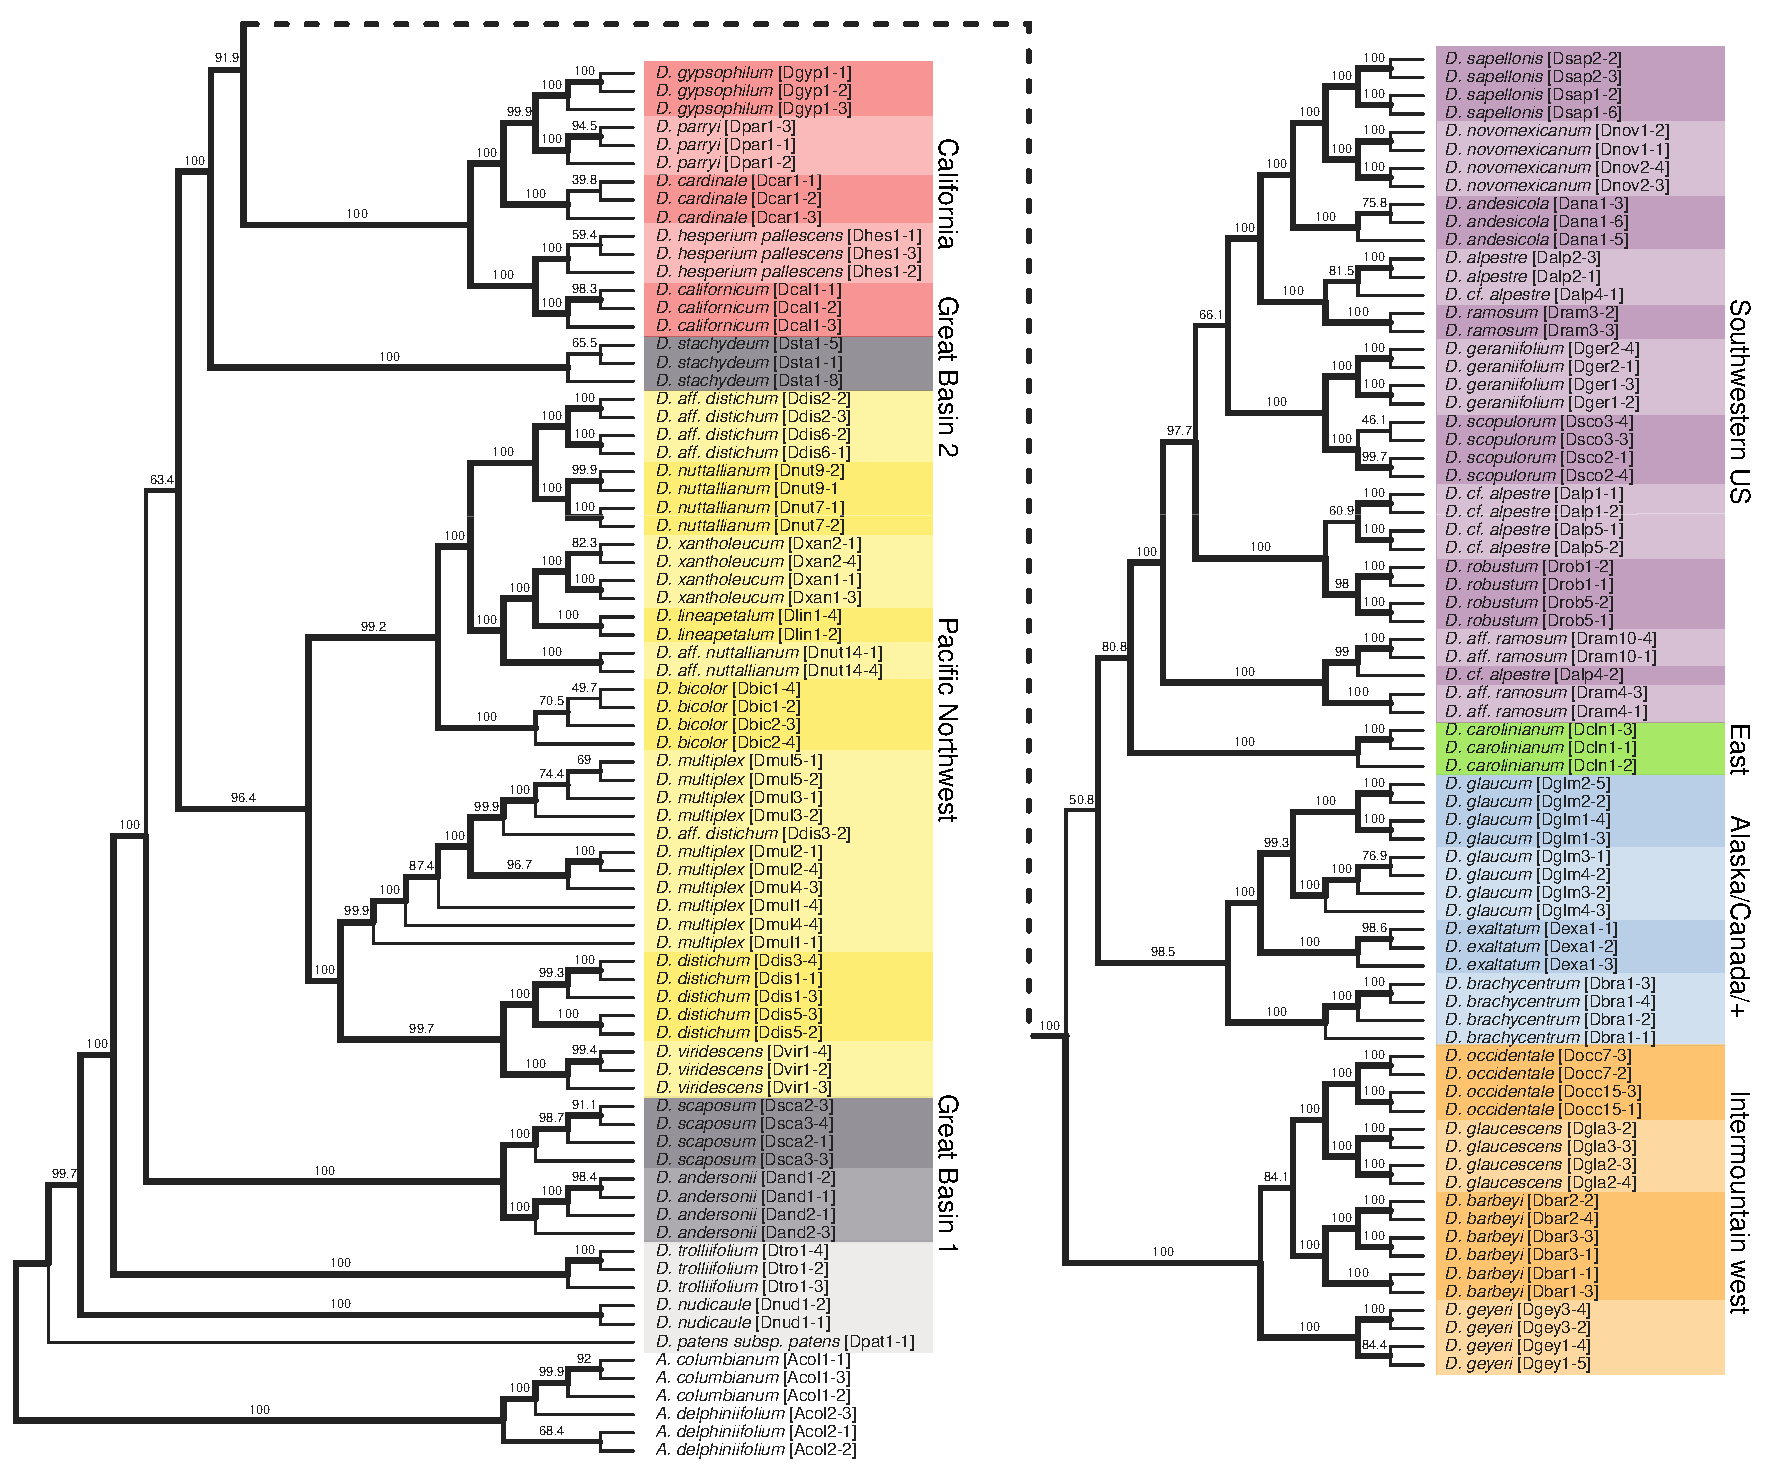
\includegraphics[width=0.99\textwidth]{./final-figures/Fig1.pdf}	
	\caption{
		A rooted phylogenetic tree for 150 samples of \emph{Delphinium} sect. \emph{Diedropetala} inferred from the min10 SNP dataset using caster. Colored rectangles highlight groups that correspond well with distinct geographic regions, representing higher-level clades. Bracketed names to the right of tips refer to sample accession numbers (see Table S1). Populations and individuals sampled from within the same taxon designation form monophyletic clades, except in a few cases involving \emph{D. distichum}, \emph{D. nuttallianum}, \emph{D. ramosum}, and \emph{D. alpestre}.
	}
	\label{fig:bigtree}
\end{figure}


\subsection{Taxonomy}
We propose a set of formal taxonomic names, following the Phylocode protocol \citep{deQueiroz2020phylo}, for the six higher-level clades containing more than one taxon that were consistently recovered across our phylogenomic analyses (Appendix 1).
To identify additional supporting evidence for these clades beyond genomics, we employed OpenAI's ChatGPT (GPT‑4) in a tool-enabled agent-based framework to retrieve and analyze morphological descriptions for each taxon. The agent performed structured searches to retrieve data from the Flora of North America \citep{Warnock_1997_FNA_Delphinium} and other authoritative referenced sources, fetching details on stem height, leaf morphology, inflorescence size, sepal color, spur length and habitat. After collating these character states, it identified synapomorphies that unite members of our specified clades, and  drafted clade definitions that highlight diagnostic characters. All data-based statements are linked to references. The process was iterative with feedback from the authors to generate etymologically appropriate names, revise formatting, and suggest additional comparisons. \textcolor{red}{Manual measurements of herbarium specimens were conducted to verify that morphological characters defined by AI were consistent for the newly defined clades.} 


%%%%%%%%%%%%%%%%%%%%%%%%%%%%%%%%%%%%%%%%%%%%%%%%%%%%%%%%%%%%%%%%%%%%%%%%%%%%%%
%%%%%%%%%%%%%%%%%%%%%%%%%%%%%%%%%%%%%%%%%%%%%%%%%%%%%%%%%%%%%%%%%%%%%%%%%%%%%%
%%%%%%%%%%%%%%%%%%%%%%%%%%%%%%%%%%%%%%%%%%%%%%%%%%%%%%%%%%%%%%%%%%%%%%%%%%%%%%
%%%%%%%%%%%%%%%%%%%%%%%%%%%%%%%%%%%%%%%%%%%%%%%%%%%%%%%%%%%%%%%%%%%%%%%%%%%%%%
%%%%%%%%%%%%%%%%%%%%%%%%%%%%%%%%%%%%%%%%%%%%%%%%%%%%%%%%%%%%%%%%%%%%%%%%%%%%%%
\section{Results}
\subsection{Genomic ddRAD sequencing and assembly}
Genomic sequencing yielded a mean of 1,071,118 (+/- S.D. 712,371) raw reads 
across all samples, which were assembled into relatively similar numbers of 
\emph{de novo} clusters within each sample (mean +/- S.D = 19,261 +/- 7,331). 
% 
We dropped samples with fewer than 1000 clusters. 
After clustering across the remaining samples and applying filters, 
the `min4' dataset included 80,169 loci, with the total alignment size of
150 samples x 6,490,732 sites (85.93\% missing) and contained 556,493 
SNPs (68.80\% missing). 
The `min10' dataset included 29,196 loci with a total alignment size of 
150 samples x 2,652,279 sites (70.96\% missing) and contained 399,001 SNPs
(58.03\% missing).


\subsection{Phylogenetic inference recovers monophyletic taxa}
\textcolor{red}{DEREN add some stuff about the ASTRAL tree and reference to its supplementary figure in this section}

All phylogenetic analyses recovered topologies showing individuals of the same 
species consistently grouped into monophyletic clades, with a few exceptions 
observed within \emph{D. distichum} Geyer ex A. Gray, \emph{D. nuttallianum} Pritzel, 
\emph{D. ramosum}, and \emph{D. alpestre} (addressed below in the context of admixture).
% 
Caster recovered the same tree topology from both the `min4' and `min10' 
datasets (Fig.~\ref{fig:bigtree}, Fig.~\ref{fig:S1}), while the ML trees
inferred by raxml-ng differed from each other, and from the caster topology.
% 
These differences are concentrated across the backbone of the tree, in the 
order of relationships among several major clades, which generally received
low support across all trees
% These differences are largely due to low backbone support affecting the ordering
% of higher-level relationships across all trees
(Fig.~\ref{fig:S2},~\ref{fig:S3}).
% 
Tree distances, measured using the generalized Robinson-Foulds mutual clustering
information metric \citep[MCI;][]{smith_information_2020}, show that the two
ML topologies share 93.3\% of information in common, while the caster topology
shares 86.0 and 91.3\% of information in common with the ML min4 and min10 
trees, respectively.

All of our tree hypotheses support three early diverging lineages that split
from the rest of our sampled \emph{Delphinium} taxa early in the radiation. 
This includes \emph{D. patens} Bentham, \emph{D. nudicaule} Torrey \& A. Gray, and \emph{D. trolliifolium} A. Gray,
which are distributed in central California, northern California, and northern 
California and the Pacific Northwest, respectively. 
We focus most of our further
analyses and discussion on the larger recovered clades in our study.
% Consider adding a final sentence here about whether we believe the 
% biogeographic implications of this.

\begin{figure}[t!]
	\centering
	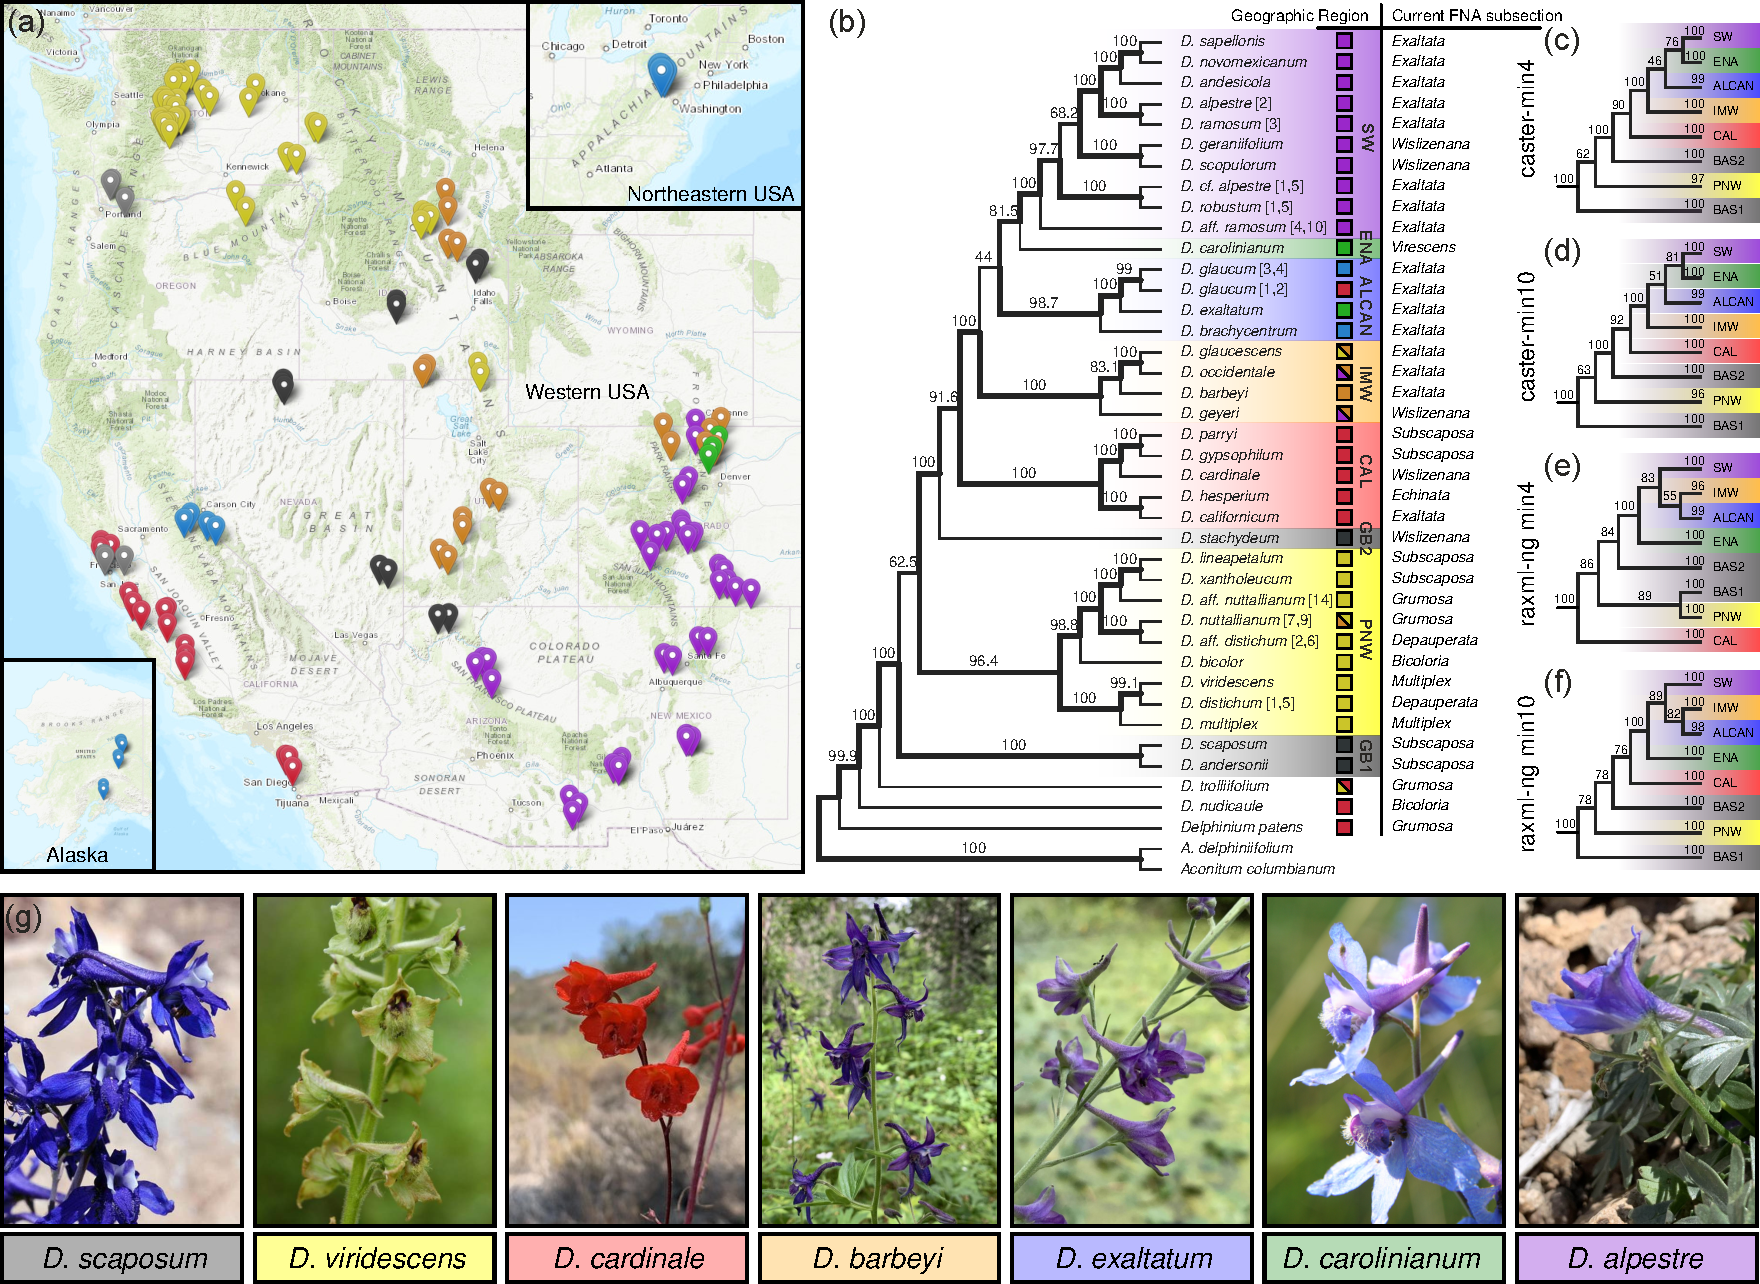
\includegraphics[width=0.95\textwidth]{./final-figures/Fig2.pdf}
	\caption{
		Phylogeny and biogeographic distribution of \emph{Delphinium} sect. \emph{Diedropetala}.
		(a) Locations of samples used in this study.	Color codes match to those used to 
		represent distinct clades in (b) that correspond closely with the following
		biogeographic regions (black: Great Basin, yellow: Pacific Northwest, red: California, orange: 
		Intermountain West, blue: Alaska and Canada, green: Eastern USA, purple: 
		Southwestern USA, gray: other).
		(b) A rooted species tree topology inferred from the min10 SNP dataset using 
		caster with population mapping of 150 individuals to 41 populations, 
		shown with local block bootstrap supports. Non-monophyletic taxa are indicated by a species-specific population number to the right of the tip name that corresponds to sample accession numbers (see Table S1).
		One or more biogeographic states occupied by each taxon are shown in a colored
		marker next to each tip.
		The current subsection designation of each taxon from the Flora of North America is
		indicated next to each tip.
		(c-f) There is substantial conflict across the backbone of the tree, which resolved into
		different topologies when analyzed using different datasets or methods.
		Support for monophyly of each clade is consistently >95\% (values at the tips
		of each tree), but support for internal splits between major clades have lower 
		support.
		(g) Images of members of \emph{Delphinium} sect. \emph{Diedropetala}. \textcolor{red}{Color of species names correspond with clades or biogeographic regions shown in (b), but the species shown are not necessarily representative of the morphological characters of their entire clade or region} (photos of \emph{D. scaposum} and \emph{D. carolinianum} from Lady Bird Johnson Wildflower Center at the University of Texas; \emph{D. viridescens} from the Burke Herbarium at the University of Washington; all others by author).
	}
	\label{fig:sptree}
\end{figure}


\subsection{Higher-level clades correspond strongly with biogeographic regions}
A set of six higher-level clades was recovered across all trees that show a strong
concordance with the following biogeographic regions: GB1 (Great Basin), PNW (Pacific Northwest), CAL (California), IMW (Intermountain West), ALCAN (Alaska/Canada), and SW (Southwestern US) (Fig.~\ref{fig:sptree}a-b).  
% 
None of these
clades corresponds uniquely with an existing taxonomic subsection in the FNA treatment (Fig.~\ref{fig:sptree}b). 
% 
Support for monophyly of each of these clades is >95\% in all trees, despite 
the fact that their ordering varies and has low support among trees
(Fig.~\ref{fig:sptree}c-f). \textcolor{red}{In addition to these six monophyletic clades, we also designated two other biogeographic regions, namely GB2 (Great Basin) and ENA (Eastern North America), but do not consider these as monophyletic clades because they are each represented by a single species only.}
% 
The grouping of regions IMW, ALCAN, ENA, and SW is consistently recovered with 
100\% support, uniting a clade that extends from Alaska to the southern Rocky
Mountains. By contrast, the phylogenetic placement of clades CAL, GB1, and GB2 has lower support, and is more variable among our inferred trees. 
% relationships among clades distributed in California 
% (CAL) and the Great Basin (GB1 and GB2) are more variable among our trees.
% 
% 
% This may be a result of admixture between species in the CAL clade and other
% early diverged lineages that also occur in California, which we examine below.
% 
% Given the uncertainty in the order of relationships among these higher-level 
% clades, and our incomplete taxon sampling, we are unable to reconstruct 
% it would be premature to draw strong
% conclusions from our results about the order and dynamics of historical biogeography
% in this clade.
% % 
% Nevertheless, our finding of strongly supported clades that correspond to distinct
% biogeographic regions represents a major revision to our understanding of the 
% phylogeny of \emph{Delphinium} sect. Diedropetala, suggesting need for a major 
% taxonomic revision.
% 
% In the following sections, we focus on elucidating the impact of hybrid admixture 
% on our phylogenetic hypotheses.

%%%%%%%%%%%%%%%%%%%%%%%%%%%%%%%%%%%%%%%%%%%% Maybe we save this section for the discussion????
% Consistent clades.
The GB1 clade occurs in the Great Basin, and is represented in our tree
by \emph{D. scaposum} Greene sampled from SE Nevada and NW Arizona, and 
\emph{D. andersonii} A. Gray sampled from southern Idaho.
% and the populations of \emph{D. andersonii} from southern Idaho. 
 % and includes \emph{D. scaposum} and
% \emph{D. andersonii}. 
% Our sampled populations of \emph{D. scaposum} are from SE Nevada and NW Arizona, 
% and the populations of \emph{D. andersonii} from southern Idaho. 
This clade does not group with the only other taxon we sampled from the Great
Basin, \emph{D. stachydeum} (A. Gray) Tidestrom, from northern Nevada, which is the sole representative of the biogeographic region designated GB2. 
% 
This split into separate regions aligns with morphological differences between these
two groups, with \textit{D. stachydeum} \textcolor{red}{exhibiting tall stems (70-150 cm), dense racemes (30-60 flowers), and distinctive fruits when compared to \textit{D. scaposum} (25-50 cm tall with 10-25 flowers per raceme) and \textit{D. andersonii} (30-60 cm tall with 10-25 flowers per raceme).} 
% 
Neither grouping corresponds to an existing taxonomic subsection, and the 
subsection names the taxa are currently assigned to are each non-monophyletic on 
our phylogeny.
% Importantly, \emph{D. scaposum} and \emph{D. andersonii} 
% are currently placed in the subsection \textit{Subscaposa} and \emph{D. stachydeum} 
% is placed in the subsection \textit{Wislizenana}, both of which have representatives
% spread across several clades of the phylogeny.

% 
The PNW clade corresponds to taxa distributed in mountainous regions in and around the Columbia
Plateau in E Washington, NE Oregon, Idaho, and W Montana. It includes \emph{D. lineapetalum} Ewan, 
\emph{D. xantholeucum} Piper, \emph{D. nuttallianum}, \emph{D. distichum}, \emph{D. bicolor} Nuttall, 
\emph{D. viridescens} Leiberg, and \emph{D. multiplex} (Ewan) C. L. Hitchcock. We recover both \emph{D. nuttallianum}
and \emph{D. distichum} as polyphyletic, possibly as a result of admixture, which we
investigate below. 
Morphologically, this clade contains several species of short‑stature that have basal
leaves and small to moderate inflorescences (3-30 flowers), but which vary in sepal
color, spur length, and seed morphology.
% 
The seven taxa in this clade are grouped into five different subsections in the 
current FNA treatment, suggesting that our results represent a major departure from
their expected relationships based on morphology.

% 
The CAL clade includes taxa distributed primarily in California, represented in our
tree by \emph{D. californicum} Torrey \& A. Gray, \emph{D. hesperium}, \emph{D. cardinale} Hook., 
\emph{D. gypsophilum} Ewan, and \emph{D. parryi} A. Gray. 
These five taxa, which have 100\% bootstrap support both as a group, and for each within-species clade, are currently placed in four different 
subsections in the current FNA treatment. \textcolor{red}{While these species all typically exhibit unwinged seeds, they have a wide range of stem height (40–160 cm), spur length (7-24 mm), and floral color (lavender‑greenish in \emph{D. californicum}, white–pink in \emph{D. gypsophilum}, dark blue in \emph{D. parryi} and \emph{D. hesperium}, and bright red in \emph{D. cardinale}). This character variation explains their current placement in different subsections, but molecular analysis indicates they are more closely related than other \textit{Delphinium} species due to geographic proximity and should be combined into the same subsection.}


The IMW clade corresponds to taxa distributed in the Intermountain West region 
between the Cascades/Sierra Nevada and the Rocky Mountains.
It is represented by four species in our study, 
\emph{D. geyeri} Greene, \emph{D. barbeyi} (Huth) Huth, \emph{D. occidentale} (S. Watson) S. Watson, and \emph{D. glaucescens} Rydberg.
These species tend to have large geographic ranges, occurring in subalpine
environments both in this region and surrounding regions.
% 
They all share a medium to large stature with moderate to large sized inflorescences of blue, purple, or white flowers with medium length (9-18 mm) spurs. 


The ALCAN clade includes \emph{D. brachycentrum} Ledebour, which is endemic to tundra environments in Alaska and northern Asia, and the widespread species \emph{D. glaucum} S. Watson, a tall larkspur whose range spans much of the North American Cordillera from Alaska and British Columbia down through the Northern Rockies, with populations also present in the Cascades and Sierra Nevada. 
Surprisingly, this group also includes \emph{D. exaltatum} Aiton, which occurs broadly in eastern North America and exhibits a disjunct pattern between the Appalachian and Ozark Mountains \citep{mohn2021exaltatum}. The two populations of \emph{D. glaucum} group monophyletically in the caster topologies, 
but \emph{D. glaucum} from Alaska groups with the \emph{D. brachycentrum} in the ML topologies.
% Members of this are all in the Exaltata subsection,
% representing the "tall larkspurs". 
Members of this clade vary in stature (the subarctic \emph{D. brachycentrum} is short) 
but are united by having glabrous to glaucous stems, moderate‑length spurs, 
paler flowers, and tending to occur in moist and rocky habitats, in contrast to 
morphologically similar, but dry adapted members of the CAL clade.

The ENA \textcolor{red}{biogeographic region} is currently represented by a single species, \emph{D. carolinianum} Walter, whose range begins east of the Rocky Mountains. Inclusion of the remaining \emph{Delphinium} taxa east of the Rockies is a vital next step that will help \textcolor{red}{redefine a clade of species from Eastern North America and} complete the phylogeny of \emph{Delphinium} sect. \emph{Diedropetala}, likely clarifying the proper relationship between \emph{D. exaltatum} and the other ALCAN species.

The SW clade is represented by eight taxa in our study which share a biogeographical
distribution throughout the southwestern United States. This includes
\emph{D. scopulorum} A. Gray, \emph{D. geraniifolium} Rydberg, \emph{D. alpestre},
\emph{D. robustum}, \emph{D. ramosum}, \emph{D. andesicola} Ewan, \emph{D. sapellonis} Tidestrom,
and \emph{D. novomexicanum} Wooton. Notably, \emph{D. ramosum} and \emph{D. alpestre}
are both polyphyletic. We recover three separate clades of \emph{D. alpestre}, each
appearing sister to a clade of \emph{D. ramosum}, or of the very morphologically
similar \emph{D. robustum}. We investigate this "replicated divergence" pattern in 
greater detail below. This group is united by all taxa having tall stature, 
large leaves and large inflorescences, with the exception of \emph{D. alpestre}, which forms a cushion habit and is only found above treeline.


%%%%%%%%%%%%%%%%%%%%%%%%%%%%%%%%%%%%%%%%%%%%%%%%%%%%%%%%%%%%%%%%%%%%%%%%%%%%%%%%%%%%%%%%
%%%%%%%%%%%%%%%%%%%%%%%%%%%%%%%%%%%%%%%%%%%%%%%%%%%%%%%%%%%%%%%%%%%%%%%%%%%%%%%%%%%%%%%%
%%%%%%%%%%%%%%%%%%%%%%%%%%%%%%%%%%%%%%%%%%%%%%%%%%%%%%%%%%%%%%%%%%%%%%%%%%%%%%%%%%%%%%%%

\subsection{Hybridization and Introgression}
Many \emph{Delphinium} species overlap in both geography and phenology in 
western North America, where numerous putative hybrids have been described.
% 
Results of our f-branch analyses confirm that genomic admixture is widespread
and common both within and between the major clades of \emph{Delphinium} that
we identified (Fig.~\ref{fig:fbranch}, Table~S2).
% 
% Across >9000 quartet tests, the mean +/- standard deviation of the 
% number of discordant SNP sites (ABBA or BABA) was 192 +/- 82 SNP
% sites per test.  
% 
Admixture is most common between taxa within the same geographically structured
clades, or between clades with overlapping geographic ranges.
% 
These patterns are consistent across alternative species tree hypotheses as well 
(Fig.~\ref{fig:S4},~\ref{fig:S5}).
% 
We suspect that some of these hypothetical introgression events may
represent false positives that can arise from non-independent signals of
admixture among multiple hybridizing taxa \citep{eaton_historical_2015, malinsky_dsuite_2021}.
Extinct and unsampled lineages may also contribute to these patterns.
% 
To avoid over-interpretation of these results, we focus below on describing 
the strongest signals of admixture, their taxonomic and geographic scope, 
and whether hybrids have been previously reported for the selected taxa 
based on observational or experimental evidence summarized in the FNA or 
Jepson Manual treatments of \emph{Delphinium}.

\begin{figure}[t!]
	\centering
	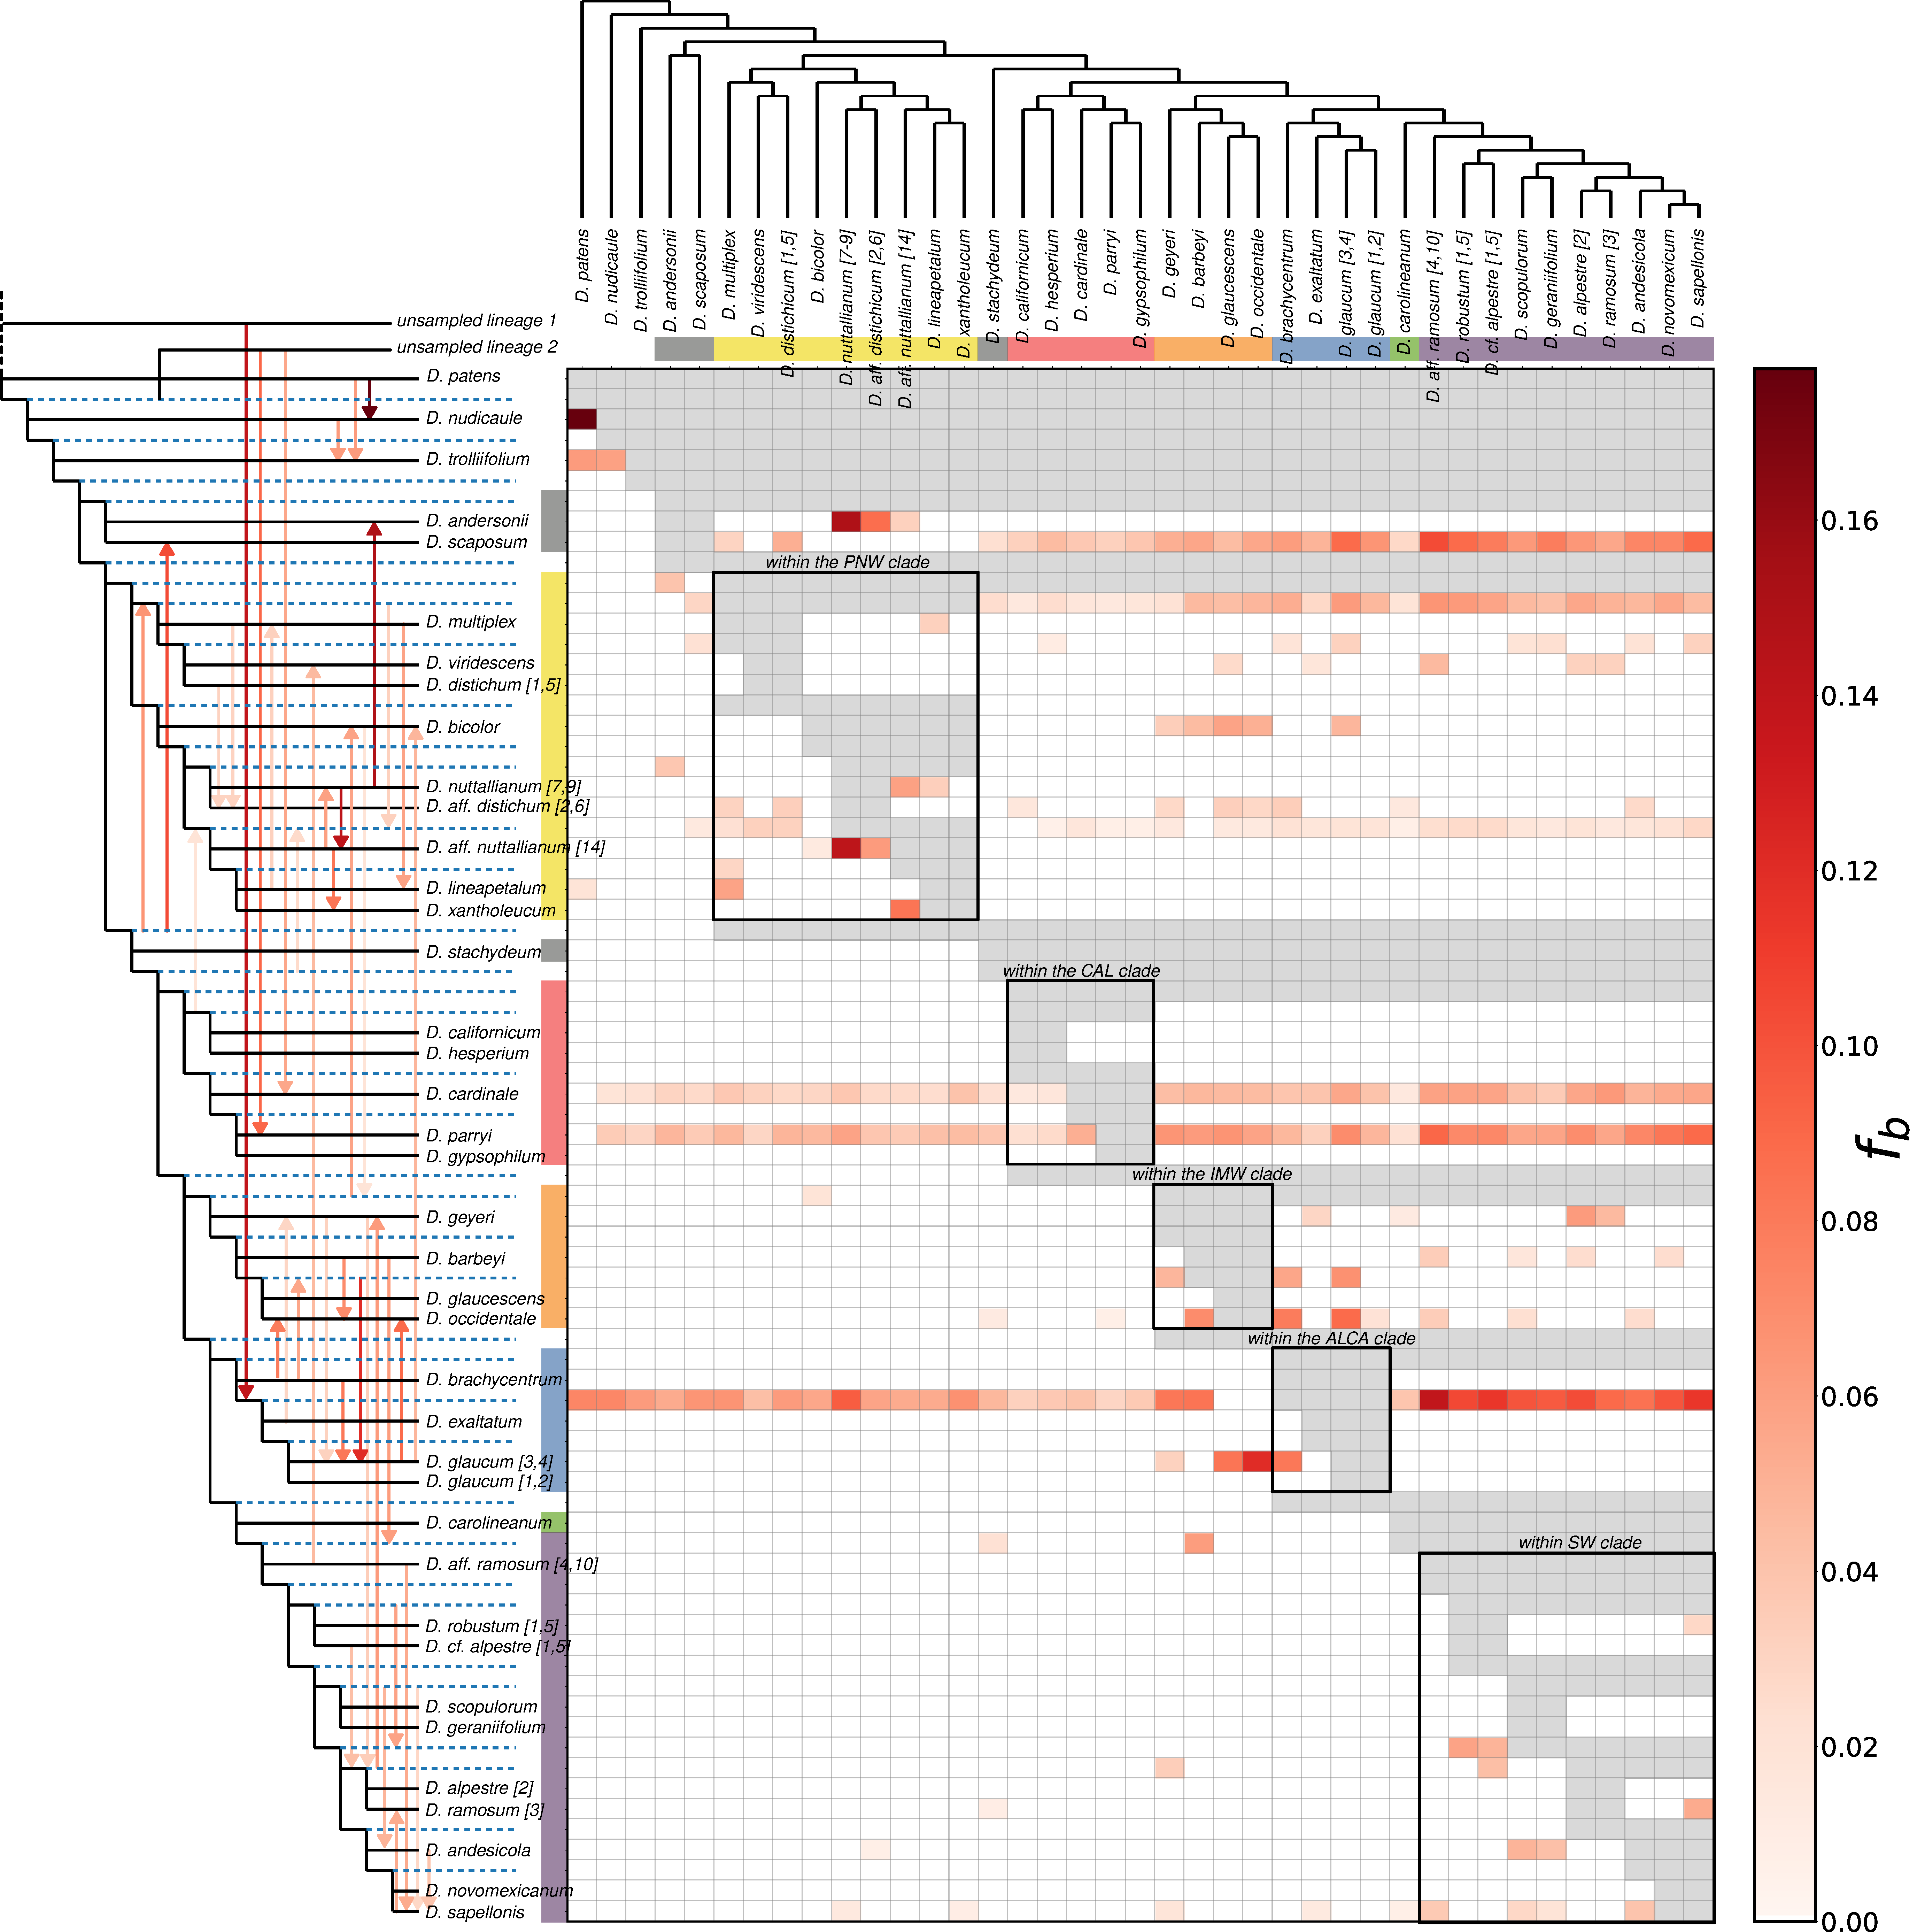
\includegraphics[width=0.95\textwidth]{./final-figures/Fig3.pdf}
	\caption{
        Heatmap of f-branch ($f_b$) statistics summarizing admixture on the reference species tree of \emph{Delphinium} sect. \emph{Diedropetala}, with
        colored blocks indicating the major clades described above.
        % 
        Columns (x-axis) correspond to donor lineages, and rows (y-axis) to putative introgressive recipient lineages. Dotted lines on the y-axis indicate internal branches of the tree.
        % , with all taxa below a dotted line belonging to that respective branch. 
        Each cell shows the excess allele sharing between the donor and the descendants of one of the recipient lineages relative to its sister lineage.
        %
        Broad bands indicate deeper introgression events, while patterns shared by one or few branches represent more recent and localized introgression.
        %
        Arrows are drawn between branches on the left tree as a hypothesized summary of the strongest admixture signals, with arrow colors representing their mean $f_b$ value. Gray boxes indicate tests that cannot be performed because they are inconsistent with the species tree topology used to generate these $f_b$ statistics. 
	}
	\label{fig:fbranch}
\end{figure}

\subsubsection{Early diverged and unsampled lineages}
The strongest signal of admixture is observed in the early diverged lineages 
represented by several taxa co-distributed in California.
The estimated admixture proportion between \emph{D. patens} and 
\emph{D. nudicaule} is approximately 17\%, while admixture between both of 
these taxa and \emph{D. trolliifolium} is approximately 6\%.
% ... while that between x and y and y and z is ...
Given their positions in the tree we cannot distinguish the directionality.
These results are consistent across multiple replicate sampled individuals
in both \emph{D. nudicaule} and \emph{D. trolliifolium}, lending increased
confidence, although we have only one representative of \emph{D. patens}. 
% 
Genomic evidence of admixture between these species is consistent with 
reported observations that both species hybridize with \emph{D. nudicaule} \citep{warnock_taxonomic_1995}.
% 
We do not find further evidence of \emph{D. nudicaule} being admixed with other taxa in our dataset, despite reports of putative hybridization with 
\emph{D. andersonii} and \emph{D. nuttallianum}.
% 

Although none of these early diverged lineages is strongly supported as a unique introgressive donor into other \emph{Delphinium} taxa in our study, they do potentially provide evidence of other \emph{unsampled} (or ghost) lineages that may be introgressive donors.
This is most notable in the clade sister to \emph{D. brachycentrum}, which includes 
the widespread taxa \emph{D. glaucum} and \emph{D. exaltatum}. 
This clade has the odd result of appearing admixed with every other sample in our 
phylogeny.
Our best hypothesis to explain this involves introgression from a divergent unsampled
lineage which we designate "unsampled lineage 1" (Fig.~\ref{fig:fbranch}). 
% 
\emph{Delphinium brachycentrum}, which lacks this signal of admixture, is the lone taxa in our
study that also occurs in Asia. If it only recently dispersed to North America, that 
could explain why this introgression event only occurred into other North American 
members of this clade.
% 
An additional ancient introgression event may have occurred into the CAL clade, 
involving \emph{D. cardinale} and/or \emph{D. parryi}, from an unsampled lineage we 
designate "unsampled lineage 2". Because this admixture signal is observed with respect to all taxa except \emph{D. patens}, we propose that it may be derived from an unsampled or ghost member of a clade that diverged between \emph{D. patens} and \emph{D. nudicaule}, and which like them, exists or existed in California. 


\subsubsection{Admixture between geographic clades}
% 
In addition to the early diverged lineages which overlap in California, there is
also evidence of introgression between several other major biogeographic
clades, particularly among members whose ranges overlap.
% 
This includes introgression between GB1 and PNW, involving \emph{D. aff. nuttallianum}
from N Utah and \emph{D. andersonii} from S Idaho. These taxa are reported to 
hybridize \citep{hickman1993jepson}, and our analyses suggest that introgression is largely unidirectional into \emph{D. andersonii}.
% 
The widespread taxon \emph{D. glaucum} also appears admixed with several lineages, 
consistent with reports that it forms many types of hybrids \citep{warnock_taxonomic_1995}.
Our genomic results confirm introgression with its close relative \emph{D. brachycentrum}, 
as well as with \emph{D. occidentale} from the IMW clade. 
The latter has been described as a hybrid between \emph{D. glaucum} and the 
IMW taxon \emph{D. barbeyi}. Although \emph{D. occidentale} appears admixed with both
species, it also shares affinity with \emph{D. glaucescens} and perhaps additional 
admixture with other taxa. Thus, our results suggest \emph{D. occidentale} has a more 
complex origin that deserves further investigation.
% 
Another taxon that appears admixed with \emph{D. glaucum} is \emph{D. bicolor},
a widespread taxon from the PNW clade, which has not been previously 
reported to hybridize. 
We do not observe admixture between \emph{D. glaucum} and \emph{D. stachydeum} 
from the GB2 clade, despite reports of hybrids between these taxa.
% 

Further evidence of introgression between divergent clades is observed between
members of the SW clade and members of both PNW and IMW, but none of these 
admixture proportions is particularly high.
% 
Although our f-branch results appear to support frequent admixture between divergent
biogeographic clades, this pattern is largely driven by a few widespread species that
hybridize abundantly, notably: \emph{D. nuttallianum} (PNW clade); 
\emph{D. barbeyi} (IMW clade); 
and \emph{D. glaucum} (ALCAN clade). 
% 
The ENA and CAL clades are relatively isolated from these widespread taxa, both 
geographically and ecologically, and are conspicuously absent of across-lineage
introgression from these frequently hybridizing taxa.

% Dnut-14 is real.
% Ddis-15 is real.
% Based on inferred patterns of introgression we are better able to interpret 
% potential taxonomic implications of our phylogenetic results.
% Our populations of \emph{D. aff. nuttallianum} (7-9) which appear highly admixed
% between 


\subsubsection{Admixture within geographic clades}

There is also abundant evidence of admixture between species within each 
biogeographic clade.
% 
For example, within the PNW clade nearly every taxon is admixed with either 
\emph{D. multiplex} or \emph{D. aff. nuttallianum}; in the IMW clade most taxa
are admixed with \emph{D. barbeyi}; and in the SW clade there is a low level of
admixture between most lineages.
% 
Given that these same taxa are widely involved in introgression between the
biogeographic clades, this suggests that alleles from nearly any species are
capable of being introgressed into another.
% 
An exception is the CAL clade, which shows little evidence of introgression between 
close relatives. 
This clade is notably characterized by high variation in flower color, 
suggesting that reproductive divergence may play an important role in 
reducing interspecies gene flow in this clade.

\section{Discussion}

\subsection{Phylogeny and Higher-level Taxonomy in \emph{Delphinium} sect. \emph{Diedropetala}}
% summarize broad results: New phylogeny with 8 geo clades and abundant admixture
We generated a large-scale genomic ddRAD-seq dataset to resolve phylogenetic 
relationships among populations and species spanning 34 taxa in the North American 
clade \emph{Delphinium} sect. \emph{Diedropetala}.
% 
Our phylogenetic results recovered most populations within taxa as monophyletic, 
and grouped all taxa into eight consistently recovered higher-level clades 
that are strongly associated with biogeographic regions.
% 
We applied a range of phylogenetic methods and data filtering approaches to examine potential impacts of missing data or methodological biases.
% 
The primary disagreement among these results involves the order in which the
eight major clades diverged across the backbone of the tree. These relationships
received low support across all trees.
% 
This is consistent with the results of f-branch statistics which indicate abundant
hybrid introgression between species both within and between many of these clades.
% 
Our new phylogenetic hypotheses for the relationships within 
\emph{Delphinium} sect. \emph{Diedropetala} present a significant advance for 
understanding the history of this North American plant clade by highlighting the dominant role of geography and hybridization in shaping its diversification.


% how does this relate to existing classifications
Our phylogenetic results conflict with existing higher-level taxonomy in 
\emph{Delphinium} sect. \emph{Diedropetala}, including the current FNA treatment.
% , which groups many taxa on the basis of morphological variation in leaf, flower, 
% and root variation.
% 
Although our study does not include complete taxon sampling, we have
included at least one representative of each subsection in the FNA treatment, 
allowing us to assess the concordance between molecular versus morphological 
similarities.
% 
Eight out of nine of the subsections in the FNA are recovered as polyphyletic
in our phylogenies, representing discordance for every subsection for which
we have more than one sample. This highlights the need for an updated taxonomy for this section in light of genomic evidence.
% 
We have assigned Phylocode-based taxon names for the six higher-level clades identified in this study that are represented by more than one species, and generated morphological descriptions for each, highlighting morphological and ecological features that unite them (Appendix 1). These formal clade definitions will aid future work aimed at re-examining our taxonomic hypotheses in light of new evidence.

\subsection{Taxonomic Revision}
\textcolor{red}{Insert taxonomic discussion and PHYLOCODE description HERE.}

\subsubsection{\textcolor{red}{Taxonomic clarification in light of admixture}}
% 
Our analyses also help to resolve long-standing disagreements 
concerning the taxonomy of multiple species. For example, we included multiple samples
of \emph{D. occidentale}, a species recognized by Ewan (\citeyear{ewan_synopsis_1945}) and Holmgren  (\citeyear{holmgren2012intermountain}), 
but which Warnock (\citeyear{warnock_taxonomic_1995}) describes as a hybrid between \emph{D. glaucum} and 
\emph{D. barbeyi}. 
% 
 Our phylogenetic results (Fig.~\ref{fig:bigtree}) show \emph{D. occidentale} as distinct from both \emph{D. barbeyi} and \emph{D. exaltatum}, and most closely related to \emph{D. glaucescens} with 100\% bootstrap support. In addition, our admixture results (Fig.~\ref{fig:fbranch}) show that while \emph{D. occidentale} is an introgressive recipient of both \emph{D. glaucum} 
and \emph{D. barbeyi}, it also appears to be an introgressive donor to multiple taxa within the PNW clade. Given that nearly all taxa in our study show some evidence of admixture, we propose that \emph{D. occidentale} is as deserving as any other taxon of species status. Our replicate population sampling, multiple phylogenomic analyses, and admixture 
analyses together provide multiple lines of genomic evidence to support previous analyses based on RAPD markers \citep{li2002genetic} and toxic alkaloids \citep{gardner_taxonomic_2002} that distinguish these three taxa from each other (for further discussion, see \emph{D. occidentale} description in Holmgren \citeyear{holmgren2012intermountain}).

\begin{figure}[t!]
	\centering
	  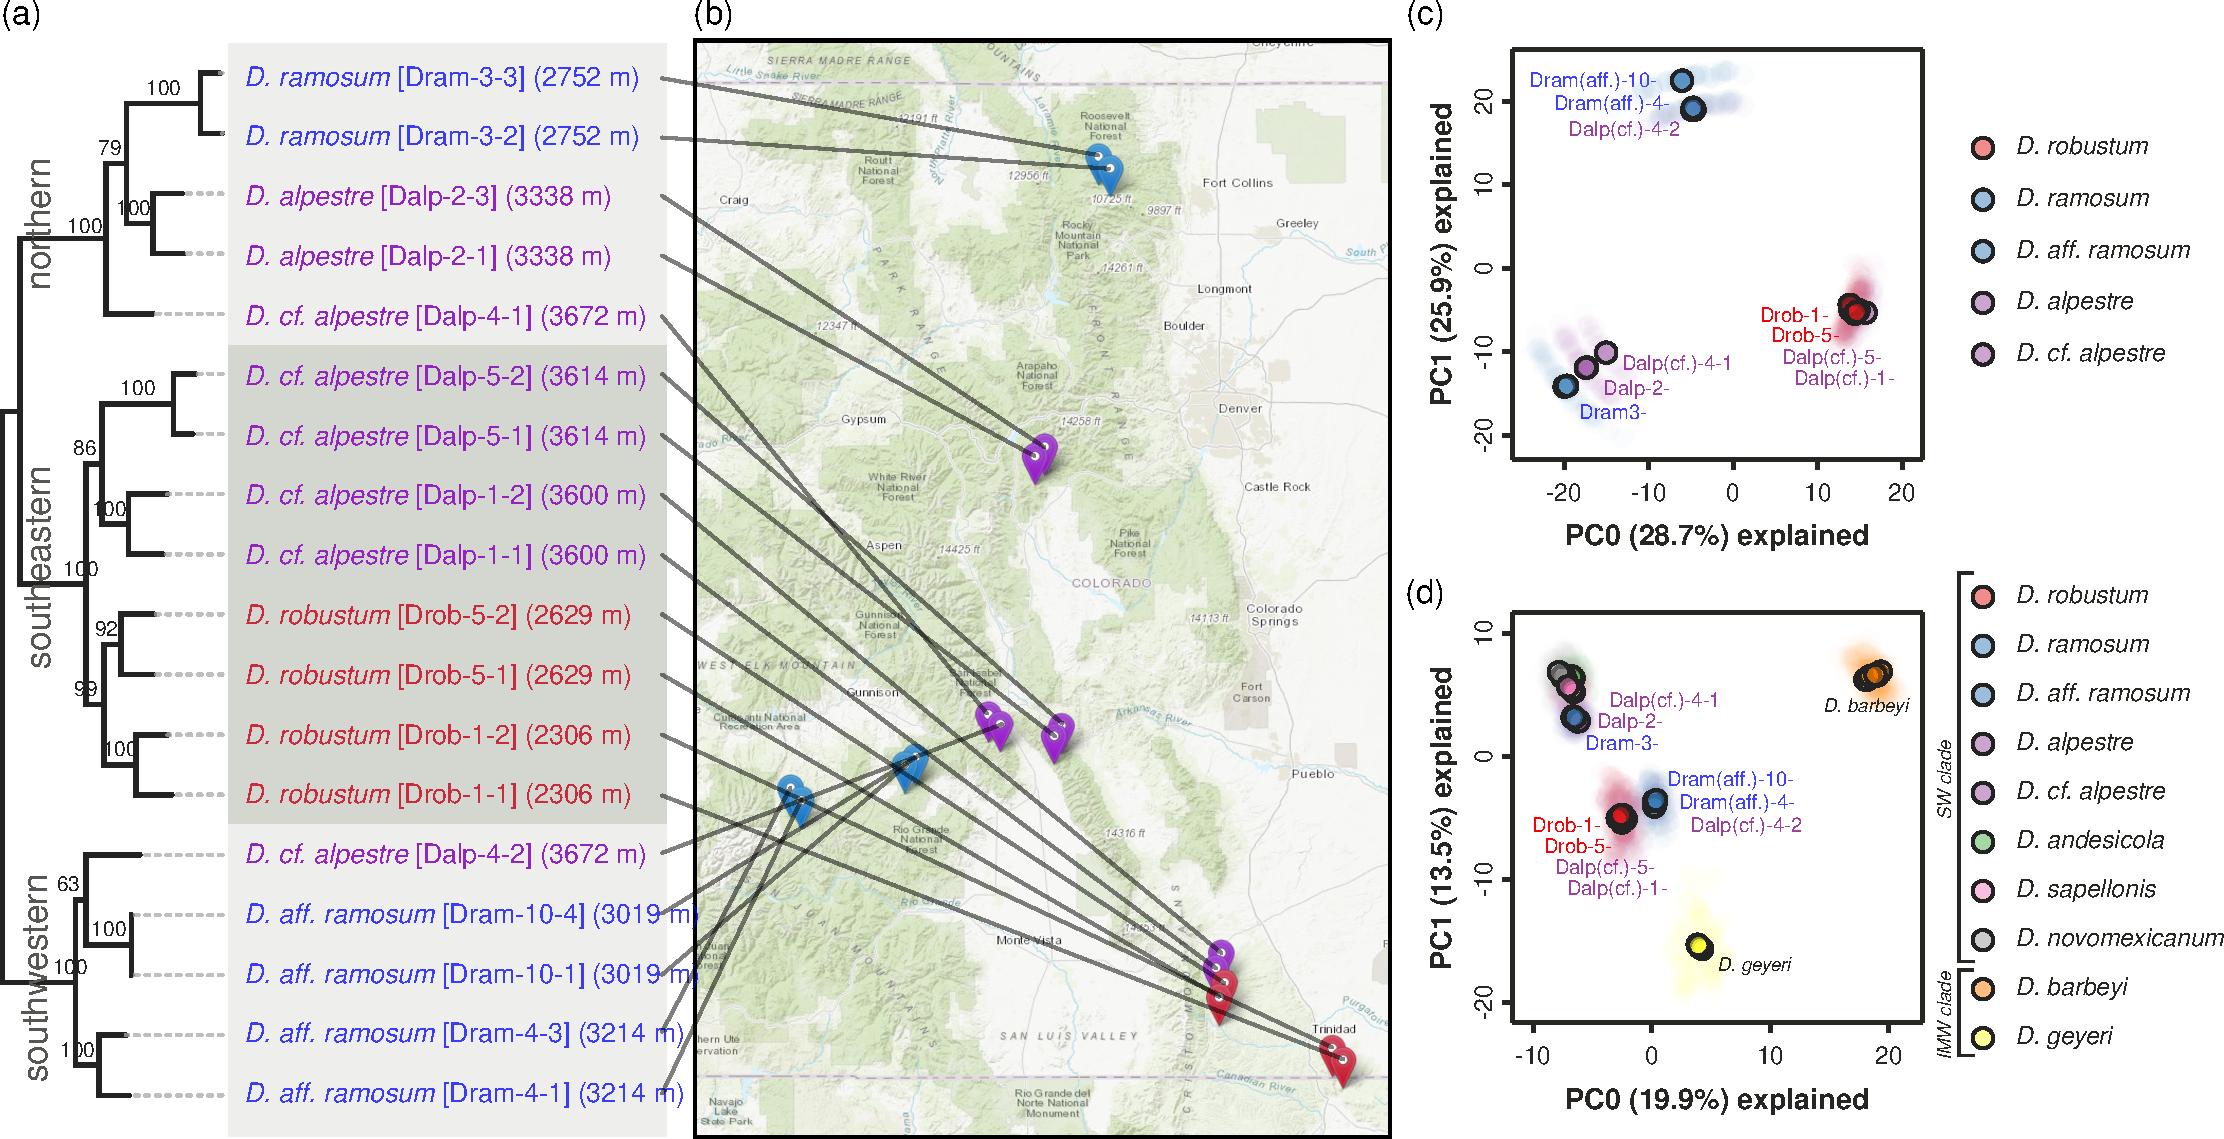
\includegraphics[width=0.99\textwidth]{./final-figures/Fig4.pdf}	
	\caption{
        Hybrid complex of \emph{D. robustum}, \emph{D. ramosum}, and \emph{D. alpestre} in the Southern Rocky Mountains. 
        (a-b) Three distinct clades are strongly supported in phylogenetic results, grouping samples by geography rather than by species determinations based on morphology.
        (c) A genomic PCA similarly groups samples by geography. Low opacity points show variation over replicate runs using randomly sampled subsets of
        unlinked SNPs. Each sample is represented by a centroid point. Labels show individual sample names, or population names when points overlap.
        (d) A genomic PCA with the inclusion of other members of the SW clade, and potential introgressive donors from the more distantly related IMW clade (\emph{D. geyeri} and \emph{D. barbeyi}). 
	}
	\label{fig:robustum}
\end{figure}

% RAMOSUM COMPLEX
There is also disagreement across floras concerning the distinction between \emph{D. ramosum}, \emph{D. robustum}, and \emph{D. alpestre}
\citep{ewan_synopsis_1945,ackerfield_flora_2022,WeberWittmann2012},
a complex of species native to Colorado and New Mexico that are grouped into our SW clade.
% 
While \emph{D. alpestre} only occurs above treeline and has a uniquely small stature, \emph{D. ramosum} and \emph{D. robustum} occur in subalpine communities and are larger and morphologically similar to each other, to the extent that \emph{D. robustum} is sometimes not recognized as a distinct taxon, and instead lumped within \emph{D. ramosum} \cite[e.g.,][]{ackerfield_flora_2022}. Importantly, on alpine summits where populations of \emph{D. alpestre} are found, there is almost always a corresponding population of one of these subalpine taxa at a lower elevation on the same mountain, leading some taxonomists to previously describe \emph{D. alpestre} as a variety of \emph{D. ramosum} (\emph{Delphinium ramosum} Rydberg var. \emph{alpestre} (Rydberg) W. A. Weber) \citep{warnock_taxonomic_1995}.


Our dataset includes multiple sampled populations of each taxon. 
% 
In phylogenetic analyses using our full dataset, both \emph{D. ramosum} and 
\emph{D. alpestre} are polyphyletic, with the high elevation \emph{D. alpestre}
resolved into three different clades (Fig.~\ref{fig:bigtree}). This pattern, along with samples from the putatively mixed Dalp4 population being split across two clades, made it difficult to assign proper placement of \emph{D. alpestre} in the species-level tree. Based on \emph{D. alpestre}'s type locality, we refer to the Dalp-2 population as true \emph{D. alpestre} and the other populations exhibiting the distinct high elevation diminutive phenotype as \emph{D. cf. alpestre}.
Similarly, we use the designations \emph{D. ramosum} and \emph{D. robustum} for
the two populations exhibiting the lower elevation phenotype in the corresponding 
geographic region where their types were originally described. 
The final \emph{D. ramosum}-like population, from the southwestern San Juan Mountains, we refer to as \emph{D. aff. ramosum}.
% 
Using a more densely subsampled sequence alignment (24 samples x 780,187 bp with 22.5\% missing data) generated for this subset of taxa, while using the CAL clade as a closer outgroup, we inferred an additional ML concatenation tree which further confirmed the phylogenetic relationships observed in the larger tree (Fig.~\ref{fig:robustum}a).
% 
This phylogeny indicates that populations of \emph{D. alpestre} are less related to each other than they are to populations of either \emph{D. ramosum} or \emph{D. robustum} at lower elevations nearby. As with the broader phylogenetic patterns in \emph{Delphinium} sect. \emph{Diedropetala}, relationships among populations within this clade match closely with geography, grouping into a northern, southeastern, and southwestern clade. These geographical clades align well with previous biochemical analysis that identified a northern and southeastern clade chemotype as distinct from a southwestern clade chemotype \citep{cook_two_2017}.  

%  
% Within each region, the population of \emph{D. alpestre} occurs at higher 
% elevations, consistent with its more diminutive stature, suggesting that this
% taxon may represent either high-elevation plasticity, or replicated adaptations
% to high elevations.

% 
We also examined patterns of ancestry among these populations using PCA performed
on 2,068 unlinked SNPs (0\% missing data) from the 18 samples in this species complex.
This also grouped samples into three distinct clusters corresponding to the same clades recovered in our phylogenetic results (Fig.~\ref{fig:robustum}c).
% 
However, when we add additional taxa representing other members of the SW clade, and
putative admixed taxa from the IMW clade, we find evidence that their relationships are shaped by admixture.
% 
A final PCA was performed on 1,792 unlinked SNPs (0\% missing) across 39 samples 
from 8 taxa (Fig.~\ref{fig:robustum}d). 
Here, the southeastern and southwestern clades from this complex both appear intermediate between a cluster formed by all other members of the SW clade, and a cluster representing \emph{D. geyeri} from the IMW clade.
% 
%Interestingly, this PCA suggests introgression occurred from \emph{D. geyeri} into these two %clades, whereas the f-branch analysis supported  results
% 
While this suggests admixture may contribute to the phylogenetic patterns in this group, it does not explain the replicated pattern of morphological divergence 
between \emph{D. cf. alpestre} and its closest relative within each subclade, as they do not differ in their patterns of admixture.
Further work is needed to investigate the role of introgression, plasticity, and adaptation in driving this replicated alpine divergence pattern.
% adaptation to an alpine environment in driving this pattern.

\subsection{Assessing an Abundance of Admixture}
Although hybridization has been frequently observed and reported in North American 
\emph{Delphinium}, our study is the first to use genomic evidence to validate 
many of these hypotheses by investigating signatures of admixture as an evolutionary consequence of hybrid introgression.
% 
Our results, based on patterns of allele sharing from thousands of genome-wide 
discordant SNPs examined in the context of phylogenetic hypotheses, show abundant 
evidence that hybrid introgression has occurred throughout the diversification of
North American \emph{Delphinium}. 
% 
Many of the strongest signals of admixture that we detected are consistent with
reports of hybridizing taxa listed in regional flora
\citep[e.g., \emph{D. patens} x \emph{D. nudicaule}; \emph{D. nuttallianum} x \emph{D. andersonii};][]{hickman1993jepson, Warnock_1997_FNA_Delphinium}, however, many other 
pairs of taxa that have been reported to hybridize do not show signals of 
admixture in our genomic results (e.g., \emph{D. nudicaule} x \emph{D. nuttallianum}).
This may indicate that some hybrids are infertile, or it may reflect that introgression is sometimes geographically localized, and occurred outside of the range of populations sampled in this study.
% 
Finally, we also detected evidence of admixture between many taxa that have not been 
previously reported to hybridize (e.g., \emph{D. glaucum} x \emph{D. bicolor}), 
identifying case studies for future investigations.

Not every hypothesized introgression event reconstructed from our f-branch results 
in Fig.~\ref{fig:fbranch} is likely to be true. Both analytical and bioinformatic
errors can inflate these estimates. Because each test examines only one quartet of taxa at a time, and different sets of taxa may share different sets of loci in RAD-seq datasets, even methods like the f-branch statistic that aim to account for the non-independence among tests may yield false positives. Nevertheless, ABBA-BABA tests have been widely applied to RAD-seq datasets \citep{heliconius_genome_consortium_butterfly_2012, eaton_inferring_2013, eaton_historical_2015, mccluskey_phylogeny_2015, vargas_conflicting_2017},
and do not typically lead to estimates of introgression nearly as abundant as observed in this study, suggesting our results are not an artifact of using anonymous genomic markers alone.
% 
Similarly, while bionformatic errors related to paralogy estimation and variant calling
can also inflate estimates of introgression, we have no reason to expect these
are inflated in our dataset. 
For example, \emph{Delphinium} is not characterized by frequent polyploidy.
% 
Karyotypes have been well studied in \emph{Delphinium} \citep{turner_cytogenetics_1992, legro_species_1961, lewis-chromosome}
where most species are diploid with a haploid chromosome number of eight (2N=16).
Among the 27/34 taxa in our study for which data is available, only \emph{D. exaltatum} is polyploid (4N=32), while all other taxa have been reported as diploids (2N=16), although four have been reported to sometimes also occur in tetraploid populations, or as tetraploid cultivars (\emph{D. gypsophilum}, \emph{D. carolinianum}, \emph{D. glaucum}, and \emph{D. geyeri}). With the exception of \emph{D. glaucum}, none of these occasionally polyploid taxa is among those most widely implicated in introgression in our results.
% % PLOIDY AND
% Reported karyotype information seems to conform with our phylogenetic results. 
% Lewis 1951 reported karyotypes for seven California species (D. hanseni, D. parishii, D. parryi, D. hesperium, D. recurvatum. D. variegatum, D. gypsophilum), which XX compared with karyotypes of X species from Oregon. They noted that the California species karyotypes are more similar to each other, as are the Oregon species to each other, than either is to species in the other region. One outlier to this was \emph{D. trolliifolium} in Oregon, which was quite different. This aligns with our phylogenetic results which found \emph{D. trolliifolium} to belong to an early diverged lineage quite distinct from other species in the Pacific Northwest.  

We have primarily interpreted our admixture results in the context of introgression. However, another potential consequence of hybridization is hybrid speciation.
% 
This process would be better modeled through alternative methods, such as network
analyses, that do not rely on a species tree hypothesis. 
% 
In this study, we are limited by the information available in short 
\emph{de novo} assembled RAD-seq loci, which individually do not 
generally contain sufficient information to infer gene trees to use as
input to common phylogenetic network inference tools \citep{solis-lemus_inferring_2016}.
% 
Thus, we were not able to confidently apply this approach to our data.
\textcolor{red}{These limitations of RAD-seq loci also inhibited us from inferring a reliable chloroplast phylogeny as a point of comparison and validation with our nuclear phylogenies.
% 
% Network-based analyses can similarly have greater power to infer unsampled
% branches, and to resolve the rooting of \emph{Delphinium} section \emph{Diedropetala}
% with respect to outgroup taxa. 
% % 
% Based on our analyses of SNPs, we proposed that introgression has occurred between
% several of our sampled lineages and unsampled or ghost lineages that we hypothesized
% the phylogenetic placement of (Fig.~\ref{fig:fbranch}). 
% % 
Although our admixture analyses have revealed many new insights into the history of 
hybridization in \emph{Delphinium}, we expect much more remains to be discovered in
future studies. 
These would benefit most by increasing taxon sampling; generating and using one or
more nuclear reference genomes for whole-genome resequencing to improve paralogy estimation and comparison with plastome phylogenies; and employing more advanced
methods for testing introgression hypotheses that can model phylogenetic networks
and make use of spatially structured patterns along chromosomes.}


\subsection{A Western North American \emph{Delphinium} Syngameon}

The term syngameon describes a set of species that are connected
by hybridization \citep{boecklen_topology_2017}. Popular examples, such as oak trees, have long been studied as both an intractable taxonomic challenge and fascinating evolutionary phenomenon, 
and recent genomic studies have only confirmed the complexity of this system \citep{eaton_historical_2015, hipp_genomic_2020, ribicoff_introgression_nodate}. 
% 
A notable feature of syngameons is that not all species hybridize evenly, yet through a network of connections -- with a few
species functioning as super-hybridizing nodes -- it is possible for genes to be exchanged, at least in theory, between any two species in the complex \citep{boecklen_topology_2017}.
% 
This is precisely the pattern that we observe in North American 
\emph{Delphinium}. Hybridization and admixture is common among co-distributed species, yet, many taxa have become differentiated across geographic and ecological space, likely due to a combination of selection and drift acting on unique and shared alleles. In addition, several widespread species, such as \emph{D. nuttallianum}, \emph{D. glaucum}, and \emph{D. barbeyi}, hybridize with species from multiple disparate geographic regions, potentially facilitating the exchange of alleles over greater geographic distances. 
% 
While this presents a challenge to many traditional methods in evolutionary systematics, such as reconstructing the biogeographic history of species, it presents many exciting opportunities as well, for reconstructing the biogeographic history of both neutral and functional alleles beyond the constraints of species barriers.
% 
% Future studies should aim to leverage this pattern to identify both parallel and convergent adaptations relevant to conservation, horticulture, and ecology.

\subsection{Conclusions}
Our phylogenomic analyses present new hypotheses and insights into the evolutionary
history of this rapidly radiated clade, and demonstrate that the divergence history
of this group is more complex than morphology alone reveals. 
% 
% Overall, 
We discover an overwhelming signal of geographically structured ancestry, 
with hybrid introgression connecting species both within and between distinct geographic regions.
% where many species co-distributed across these regions also carry clear signals of admixture.
% 
Future work should include the remaining unsampled taxa to better address questions concerning the origin and early dispersal history of \emph{Delphinium} upon its arrival in North America, including diversification patterns linked to climatic, topographical, and pollination shifts. Towards this goal, our phylogenetic revision of \emph{Delphinium} sect. \emph{Deidropetala} represents a major advance for understanding  the evolutionary history of this enigmatic North American plant clade.

% Future work should include the remaining unsampled taxa so that questions concerning biogeographic history, dispersal, and diversification linked to climatic, topographical, or pollination shifts (Sharma et al., 2024) since \emph{Delphinium}’s arrival to North America can be tested. While a full sampling of all \emph{Delphinium} sect. \emph{Diedropetala} species is required, the need for a major revision of higher-level taxonomy within this clade is clear, which should aim to identify morphological characteristics among species that are concordant with the monophyletic clades supported by molecular evidence.

\subsection{Acknowledgments}
This work was supported by the National Science Foundation (NSF DEB-2046813 awarded to DARE) and a Graduate Research Fellowship from the Botanical Society of America (awarded to JBM). Thanks to Richard Ree, Sarah Jacobs, Mike Hickerson, and Maria Uriarte for feedback.

\subsection{Competing Interests} 
None.

\subsection{Author Contributions}
JBM, DARE, and DC planned and designed the research. JBM and DC conducted fieldwork. BSB and KT conducted molecular labwork. JBM and DARE analyzed the data and wrote the manuscript.


\subsection{Data Availability}
Sequence data is available on the NCBI sequence read archive under project identifier PRNJXXX. Phylip formatted sequence alignment files and newick formatted tree files are available on DRYAD (\url{http://datadryad.org/share/LINK_NOT_FOR_PUBLICATION/UvAYjrrXFMkhJwDy8OlkOFIqvD3nMXAJ0NaN1rqV6ek}).


\bibliographystyle{ecol_let}
\bibliography{references}  


\beginsupplement

\begin{figure}[p]
	\centering
    %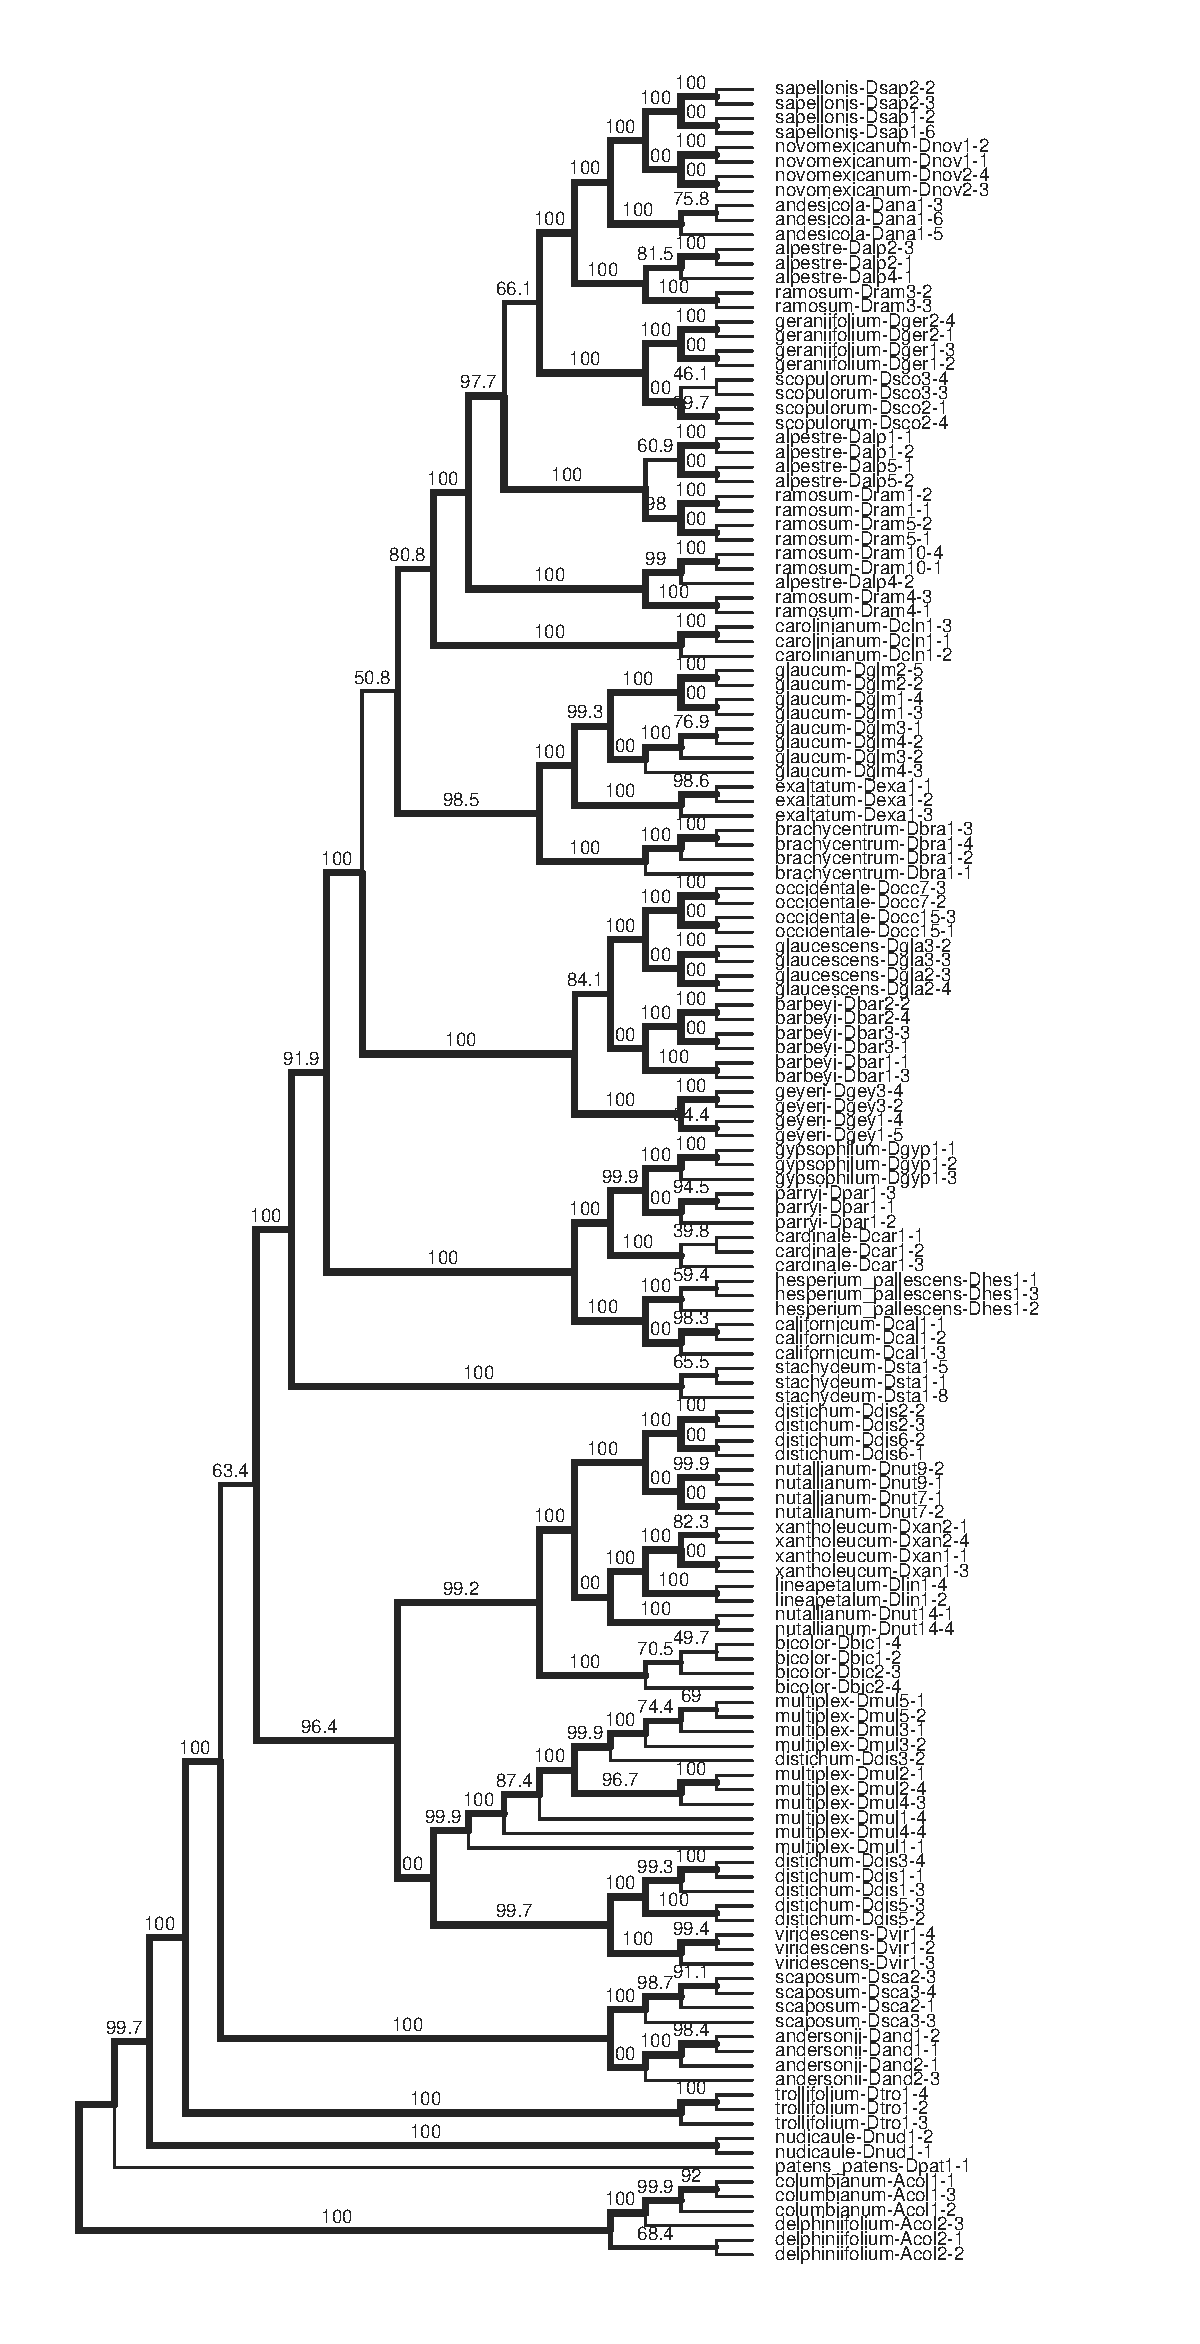
\includegraphics[width=0.95\textwidth] {./final-figures/FigS1.pdf}
      
	\caption{
		A rooted phylogenetic tree for 150 samples of \emph{Delphinium} sect. \emph{Diedropetala}
		inferred from the min4 SNP dataset using caster, with supports shown from
		1000 local block bootstrap replicates. 
		Colored rectangles highlight
		groups that correspond well with discrete geographic regions, representing higher-level 
		clades. Replicate samples within each taxon form monophyletic clades, except in the case
		of \emph{D. distichum}, \emph{D. nuttallianum}, \emph{D. rasomum}, and \emph{D. alpestre}.
	}
	\label{fig:S1}
\end{figure}

\begin{figure}[p]
	\centering
	% 
\includegraphics[width=0.95\textwidth]{./figures/FigS2.pdf}
	\caption{
		A rooted phylogenetic tree for 150 samples of \emph{Delphinium} sect. \emph{Diedropetala}
		inferred from the min4 sequence alignment using raxml-ng, with supports shown from
		200 non-parametric bootstrap replicates. 
		Colored rectangles highlight
		groups that correspond well with discrete geographic regions, representing higher-level 
		clades. Replicate samples within each taxon form monophyletic clades, except in the case
		of \emph{D. distichum}, \emph{D. nuttallianum}, \emph{D. rasomum}, and \emph{D. alpestre}.
	}
	\label{fig:S2}
\end{figure}

\begin{figure}[p]
	\centering
	% 
\includegraphics[width=0.95\textwidth]{./figures/FigS3.pdf}
	\caption{
		A rooted phylogenetic tree for 150 samples of \emph{Delphinium} sect. \emph{Diedropetala}
		inferred from the min10 sequence alignment using raxml-ng, with supports shown from
		200 non-parametric bootstrap replicates. 
		Colored rectangles highlight
		groups that correspond well with discrete geographic regions, representing higher-level 
		clades. Replicate samples within each taxon form monophyletic clades, except in the case
		of \emph{D. distichum}, \emph{D. nuttallianum}, \emph{D. rasomum}, and \emph{D. alpestre}.
	}
	\label{fig:S3}
\end{figure}


\begin{figure}[p]
	\centering
	% 
\includegraphics[width=0.95\textwidth]{./figures/FigS4.pdf}
	\caption{
		f-branch analysis of admixture performed on the raxml-min4 species tree hypothesis.	
	}
	\label{fig:S4}
\end{figure}

\begin{figure}[p]
	\centering
	% 
\includegraphics[width=0.95\textwidth]{./figures/FigS5.pdf}
	\caption{
		f-branch analysis of admixture performed on the raxml-min10 species tree hypothesis.
	}
	\label{fig:S5}
\end{figure}

\begin{table}[p]
	\centering
	% \includegraphics[width=0.95\textwidth]{./figures/TableS1.csv}
	\caption{
		Plant accessions used in this study with GPS coordinates and sample identifiers for vouchers stored at the USDA-ARS Poisonous Plant Research Laboratory in Logan, UT.
	}
	\label{fig:TableS1}
\end{table}

\begin{table}[p]
	\centering
	% \includegraphics[width=0.95\textwidth]{./figures/TableS2.tsv}
	\caption{
		Dsuite f-branch analysis results performed on the caster min10 41-tip species tree hypothesis.
	}
	\label{fig:TableS2}
\end{table}



\end{document}

